\documentclass[fleqn,10pt]{article}
\usepackage[utf8]{inputenc}
\usepackage[T1]{fontenc}
\usepackage[left=2cm,right=2cm,top=2.25cm,bottom=2.25cm,headheight=12pt,letterpaper]{geometry}
\usepackage{subcaption, graphicx, pgfplots, tikz, siunitx}
\usepackage[labelfont={bf,sf},labelsep=period,justification=raggedright]{caption}
\usepackage[explicit]{titlesec}
\usepackage[colorlinks=true, allcolors=blue]{hyperref}
\usetikzlibrary{scopes, backgrounds, matrix, shapes.geometric, patterns,
    decorations.markings, arrows.meta, calc, positioning}

\renewcommand{\familydefault}{\sfdefault}

\pgfplotsset{compat=1.18}

\definecolor{color1}{RGB}{0,0,0}
\titleformat{\section}
  {\color{color1}\large\sffamily\bfseries}
  {\thesection}
  {0.5em}
  {#1}
  []
\titleformat{name=\section,numberless}
  {\color{color1}\large\sffamily\bfseries}
  {}
  {0em}
  {#1}
  []
\titleformat{\subsection}
  {\sffamily\bfseries}
  {\thesubsection}
  {0.5em}
  {#1}
  []
\titlespacing*{\section}{0pc}{3ex plus 4pt minus 3pt}{5pt}
\titlespacing*{\subsection}{0pc}{2.5ex plus 3pt minus 2pt}{0pt}

\definecolor{cb_black}{RGB}{0,0,0}
\definecolor{cb_sky_blue}{RGB}{86,180,233}
\definecolor{cb_yellow}{RGB}{240,228,66}
\definecolor{cb_reddish_purple}{RGB}{204,121,167}
\definecolor{cb_vermillion}{RGB}{213,94,0}
\definecolor{cb_blue}{RGB}{2,112,189}
\definecolor{hs_blue}{RGB}{51,51,255}
\definecolor{imu_green}{RGB}{0,255,0}
\definecolor{cb_orange}{RGB}{229,126,34}
\definecolor{cb_green}{RGB}{113,178,112}
\definecolor{cb_dark_gray}{RGB}{102,102,102}
\definecolor{cb_gray}{RGB}{102,102,102}

\pgfplotsset{
    every axis/.append style={
        axis x line=bottom,
        axis y line=left,
        label style={font=\bfseries},
        tick label style={font=\small},
        legend style={font=\small},
        grid=major,
        grid style={dashed, gray!50},
    }
}

\begin{document}

\vspace*{\fill}
\begin{center}
{\LARGE\bfseries Supplementary Information}\\[12pt]
{\large Truly Mobile Sub-Terahertz Communications Beyond 6G\\[4pt]via Just-in-Time IMU-Assisted Beam Management}
\end{center}
\vspace*{\fill}

\newpage


\section*{Establishing Boundaries for IMU Sensor Data}
To establish realistic parameters for the mobility scenarios used in this paper, we conducted two experiments to capture typical human motion profiles. An IMU was affixed to a smartphone case to record its motion during common user activities. The first experiment (Supplementary Fig.~1) captures a phone-raising gesture, consisting of lifting the device from rest to ear level to simulate answering a phone call and then lowering it back down, repeated twice. This hybrid motion combines both translational and rotational components, producing translational accelerations exceeding \SI{10}{m/s^2} and rotational velocities up to \SI{200}{\degree/s}.

\begin{figure}[h!]
    \centering
    \begin{subfigure}{0.99\linewidth}
        \centering
        \include{Figures/SuppFig1a}
        \vspace{-34pt}
        \caption{Translational acceleration.}
    \end{subfigure}

    \begin{subfigure}{0.99\linewidth}
        \centering
        \include{Figures/SuppFig1b}
        \vspace{-34pt}
        \caption{Rotational acceleration.}
    \end{subfigure}
    \caption{IMU measurements for the phone-raising gesture (lift to ear level and lower), repeated twice. Subfigures show (a)~translational acceleration and (b)~rotational acceleration over time.}
    \vspace{-5pt}
\end{figure}

The second experiment (Supplementary Fig.~2) isolates rotational-dominant motion by capturing a \SI{90}{\degree} body turn followed by a return to the original orientation, repeated twice. Here, rotational velocities are comparable to those observed in the first experiment, but translational accelerations remain low, driven primarily by centripetal forces.

\begin{figure}[h!]
    \centering
    \begin{subfigure}{0.99\linewidth}
        \centering
        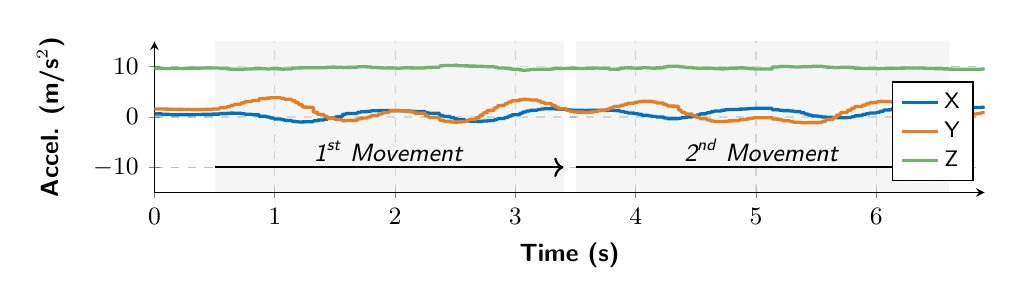
\begin{tikzpicture}
    \begin{axis}[
        width=\linewidth, height=3.5cm,
        xlabel={Time (s)},
        ylabel={Accel. (m/s$^2$)},
        ylabel style={font=\scriptsize\bfseries},
        yticklabel style={
            align=right,
            text width=2em,
        },
        xmin=0, xmax=6.9,
        ymin=-15, ymax=15,
        grid=major,
        grid style={dashed, gray!50},
        legend style={
            at={(axis description cs:1,0)},
            anchor=south east,
            nodes={scale=0.9, transform shape},
            legend cell align=left,
            xshift=-4pt,
            yshift=4pt,
        },
        legend image post style={scale=0.75},
        tick label style={font=\small},
        label style={font=\small\bfseries},
        y filter/.code={\pgfmathparse{\pgfmathresult*9.80665}},
    ]
        \pgfplotsextra{
    \fill[gray!15, opacity=0.5] (axis cs:0.5, \pgfkeysvalueof{/pgfplots/ymin}) rectangle (axis cs:3.4, \pgfkeysvalueof{/pgfplots/ymax});
    \draw[->, black, thick] (axis cs:0.5, -10) -- (axis cs:3.4, -10);
    \node[above, font=\small, text width=2.5cm, align=center, inner sep=2pt] at (axis cs:1.95, -10) {\textit{1\textsuperscript{st} Movement}};

    \fill[gray!15, opacity=0.5] (axis cs:3.5, \pgfkeysvalueof{/pgfplots/ymin}) rectangle (axis cs:6.6, \pgfkeysvalueof{/pgfplots/ymax});
    \draw[->, black, thick] (axis cs:3.5, -10) -- (axis cs:6.6, -10);
    \node[above, font=\small, text width=2.5cm, align=center, inner sep=2pt] at (axis cs:5.05, -10) {\textit{2\textsuperscript{nd} Movement}};
}
        \addplot+[color=cb_blue, mark=none, solid, very thick, line join=round]
            coordinates {
                (0.000, 0.068) (0.000, 0.067) (0.000, 0.066) (0.000, 0.065) (0.000, 0.065) (0.000, 0.064) (0.000, 0.063) (0.000, 0.062) (0.060, 0.062) (0.060, 0.061) (0.060, 0.060) (0.060, 0.059) (0.060, 0.059) (0.060, 0.058) (0.060, 0.058) (0.060, 0.057) (0.090, 0.056) (0.090, 0.056) (0.090, 0.055) (0.090, 0.055) (0.090, 0.054) (0.090, 0.054) (0.090, 0.053) (0.090, 0.053) (0.121, 0.052) (0.121, 0.052) (0.121, 0.052) (0.121, 0.051) (0.121, 0.051) (0.121, 0.051) (0.121, 0.050) (0.121, 0.050) (0.150, 0.050) (0.150, 0.049) (0.150, 0.049) (0.150, 0.049) (0.150, 0.049) (0.150, 0.049) (0.150, 0.048) (0.150, 0.048) (0.180, 0.048) (0.180, 0.048) (0.180, 0.048) (0.180, 0.048) (0.180, 0.048) (0.180, 0.047) (0.180, 0.047) (0.180, 0.047) (0.241, 0.047) (0.241, 0.047) (0.241, 0.047) (0.241, 0.047) (0.241, 0.047) (0.241, 0.047) (0.241, 0.047) (0.241, 0.047) (0.302, 0.047) (0.302, 0.047) (0.302, 0.047) (0.302, 0.047) (0.302, 0.048) (0.302, 0.048) (0.302, 0.048) (0.302, 0.048) (0.302, 0.048) (0.302, 0.048) (0.302, 0.048) (0.302, 0.048) (0.302, 0.049) (0.302, 0.049) (0.302, 0.049) (0.302, 0.049) (0.361, 0.049) (0.361, 0.049) (0.361, 0.050) (0.361, 0.050) (0.361, 0.050) (0.361, 0.050) (0.361, 0.050) (0.361, 0.051) (0.390, 0.051) (0.390, 0.051) (0.390, 0.051) (0.390, 0.052) (0.390, 0.052) (0.390, 0.052) (0.390, 0.052) (0.390, 0.053) (0.422, 0.053) (0.422, 0.053) (0.422, 0.053) (0.422, 0.054) (0.422, 0.054) (0.422, 0.054) (0.422, 0.055) (0.422, 0.055) (0.481, 0.055) (0.481, 0.055) (0.481, 0.056) (0.481, 0.056) (0.481, 0.056) (0.481, 0.057) (0.481, 0.057) (0.481, 0.058) (0.540, 0.058) (0.540, 0.059) (0.540, 0.059) (0.540, 0.059) (0.540, 0.060) (0.540, 0.060) (0.540, 0.061) (0.540, 0.061) (0.541, 0.062) (0.541, 0.063) (0.541, 0.063) (0.541, 0.064) (0.541, 0.065) (0.541, 0.065) (0.541, 0.066) (0.541, 0.067) (0.601, 0.067) (0.601, 0.068) (0.601, 0.068) (0.601, 0.069) (0.601, 0.070) (0.601, 0.071) (0.601, 0.072) (0.601, 0.072) (0.631, 0.073) (0.631, 0.074) (0.631, 0.075) (0.631, 0.075) (0.631, 0.076) (0.631, 0.076) (0.632, 0.077) (0.632, 0.077) (0.661, 0.077) (0.661, 0.077) (0.661, 0.077) (0.661, 0.077) (0.661, 0.077) (0.662, 0.076) (0.662, 0.076) (0.662, 0.075) (0.720, 0.074) (0.721, 0.074) (0.721, 0.073) (0.721, 0.072) (0.721, 0.071) (0.721, 0.070) (0.721, 0.068) (0.721, 0.067) (0.751, 0.066) (0.751, 0.065) (0.751, 0.063) (0.751, 0.062) (0.751, 0.060) (0.751, 0.059) (0.751, 0.058) (0.751, 0.056) (0.810, 0.055) (0.810, 0.053) (0.810, 0.052) (0.810, 0.050) (0.810, 0.049) (0.810, 0.047) (0.810, 0.045) (0.810, 0.044) (0.869, 0.042) (0.870, 0.041) (0.870, 0.039) (0.870, 0.038) (0.870, 0.036) (0.870, 0.034) (0.870, 0.033) (0.870, 0.031) (0.870, 0.029) (0.870, 0.027) (0.870, 0.025) (0.870, 0.023) (0.870, 0.022) (0.870, 0.020) (0.870, 0.018) (0.871, 0.016) (0.930, 0.015) (0.930, 0.013) (0.930, 0.012) (0.930, 0.010) (0.930, 0.008) (0.930, 0.006) (0.930, 0.004) (0.930, 0.002) (0.959, -0.001) (0.959, -0.003) (0.960, -0.006) (0.960, -0.009) (0.960, -0.012) (0.960, -0.014) (0.960, -0.017) (0.960, -0.020) (0.992, -0.023) (0.992, -0.026) (0.992, -0.029) (0.992, -0.031) (0.992, -0.034) (0.992, -0.036) (0.992, -0.038) (0.992, -0.040) (1.052, -0.042) (1.053, -0.044) (1.053, -0.045) (1.053, -0.047) (1.053, -0.049) (1.053, -0.050) (1.053, -0.052) (1.053, -0.054) (1.081, -0.055) (1.081, -0.057) (1.081, -0.059) (1.081, -0.061) (1.081, -0.063) (1.081, -0.065) (1.081, -0.067) (1.081, -0.069) (1.141, -0.071) (1.141, -0.074) (1.141, -0.076) (1.141, -0.078) (1.141, -0.080) (1.141, -0.082) (1.141, -0.084) (1.141, -0.086) (1.170, -0.088) (1.170, -0.089) (1.170, -0.091) (1.170, -0.092) (1.170, -0.094) (1.170, -0.095) (1.170, -0.096) (1.170, -0.097) (1.200, -0.098) (1.200, -0.099) (1.200, -0.100) (1.200, -0.100) (1.200, -0.101) (1.200, -0.101) (1.200, -0.101) (1.200, -0.101) (1.231, -0.101) (1.231, -0.101) (1.231, -0.101) (1.231, -0.101) (1.231, -0.100) (1.231, -0.100) (1.231, -0.100) (1.231, -0.099) (1.320, -0.098) (1.320, -0.098) (1.320, -0.097) (1.320, -0.096) (1.320, -0.095) (1.320, -0.094) (1.320, -0.093) (1.320, -0.092) (1.321, -0.090) (1.321, -0.089) (1.321, -0.087) (1.321, -0.086) (1.321, -0.084) (1.321, -0.082) (1.321, -0.081) (1.321, -0.079) (1.356, -0.077) (1.356, -0.076) (1.356, -0.074) (1.356, -0.072) (1.356, -0.070) (1.356, -0.068) (1.356, -0.066) (1.357, -0.064) (1.411, -0.062) (1.411, -0.060) (1.411, -0.058) (1.411, -0.056) (1.411, -0.054) (1.411, -0.051) (1.411, -0.049) (1.411, -0.046) (1.440, -0.044) (1.440, -0.041) (1.440, -0.039) (1.440, -0.036) (1.440, -0.034) (1.440, -0.031) (1.440, -0.028) (1.440, -0.025) (1.500, -0.022) (1.500, -0.019) (1.500, -0.016) (1.500, -0.013) (1.500, -0.010) (1.501, -0.006) (1.501, -0.003) (1.501, 0.000) (1.560, 0.004) (1.560, 0.007) (1.560, 0.011) (1.560, 0.014) (1.560, 0.018) (1.560, 0.021) (1.560, 0.025) (1.561, 0.028) (1.561, 0.031) (1.561, 0.034) (1.561, 0.037) (1.561, 0.040) (1.561, 0.043) (1.561, 0.046) (1.561, 0.049) (1.561, 0.051) (1.591, 0.054) (1.591, 0.056) (1.591, 0.059) (1.591, 0.061) (1.591, 0.063) (1.591, 0.065) (1.591, 0.067) (1.591, 0.069) (1.684, 0.071) (1.684, 0.072) (1.684, 0.074) (1.684, 0.075) (1.684, 0.077) (1.684, 0.078) (1.684, 0.080) (1.684, 0.081) (1.685, 0.082) (1.685, 0.084) (1.685, 0.085) (1.685, 0.086) (1.685, 0.088) (1.685, 0.089) (1.685, 0.091) (1.685, 0.092) (1.711, 0.094) (1.711, 0.095) (1.711, 0.097) (1.712, 0.098) (1.712, 0.099) (1.712, 0.101) (1.712, 0.102) (1.712, 0.104) (1.771, 0.105) (1.771, 0.107) (1.771, 0.108) (1.771, 0.109) (1.771, 0.111) (1.771, 0.112) (1.771, 0.114) (1.771, 0.115) (1.802, 0.116) (1.802, 0.118) (1.802, 0.119) (1.802, 0.120) (1.802, 0.121) (1.802, 0.122) (1.802, 0.123) (1.802, 0.124) (1.863, 0.125) (1.863, 0.126) (1.863, 0.127) (1.863, 0.128) (1.863, 0.128) (1.863, 0.129) (1.863, 0.129) (1.863, 0.129) (1.893, 0.130) (1.894, 0.130) (1.894, 0.131) (1.894, 0.131) (1.894, 0.131) (1.894, 0.131) (1.894, 0.131) (1.894, 0.131) (1.950, 0.131) (1.950, 0.131) (1.950, 0.130) (1.951, 0.129) (1.951, 0.129) (1.951, 0.128) (1.951, 0.127) (1.951, 0.127) (1.956, 0.126) (1.956, 0.126) (1.956, 0.126) (1.956, 0.126) (1.956, 0.127) (1.956, 0.127) (1.956, 0.127) (1.956, 0.128) (2.013, 0.128) (2.013, 0.128) (2.013, 0.129) (2.013, 0.129) (2.013, 0.129) (2.013, 0.129) (2.013, 0.129) (2.013, 0.129) (2.040, 0.129) (2.040, 0.129) (2.040, 0.128) (2.040, 0.128) (2.040, 0.128) (2.040, 0.127) (2.040, 0.126) (2.040, 0.126) (2.071, 0.125) (2.071, 0.124) (2.071, 0.123) (2.071, 0.123) (2.071, 0.122) (2.071, 0.121) (2.071, 0.120) (2.071, 0.120) (2.132, 0.119) (2.132, 0.118) (2.132, 0.118) (2.132, 0.117) (2.132, 0.117) (2.132, 0.116) (2.132, 0.116) (2.132, 0.115) (2.161, 0.115) (2.161, 0.114) (2.161, 0.113) (2.161, 0.113) (2.161, 0.112) (2.161, 0.111) (2.161, 0.110) (2.161, 0.109) (2.251, 0.108) (2.251, 0.107) (2.251, 0.106) (2.251, 0.105) (2.251, 0.104) (2.251, 0.102) (2.251, 0.101) (2.251, 0.100) (2.251, 0.098) (2.251, 0.097) (2.251, 0.095) (2.251, 0.094) (2.251, 0.093) (2.251, 0.091) (2.251, 0.090) (2.251, 0.088) (2.279, 0.087) (2.279, 0.085) (2.279, 0.083) (2.279, 0.082) (2.279, 0.080) (2.279, 0.078) (2.279, 0.076) (2.279, 0.074) (2.370, 0.072) (2.370, 0.069) (2.370, 0.067) (2.370, 0.064) (2.370, 0.062) (2.370, 0.059) (2.370, 0.057) (2.370, 0.054) (2.372, 0.051) (2.372, 0.048) (2.372, 0.045) (2.372, 0.042) (2.372, 0.039) (2.372, 0.036) (2.372, 0.033) (2.372, 0.030) (2.401, 0.027) (2.402, 0.024) (2.402, 0.022) (2.402, 0.019) (2.402, 0.017) (2.402, 0.014) (2.402, 0.011) (2.402, 0.009) (2.462, 0.006) (2.462, 0.004) (2.462, 0.001) (2.462, -0.002) (2.462, -0.005) (2.462, -0.007) (2.462, -0.011) (2.462, -0.014) (2.491, -0.017) (2.491, -0.020) (2.491, -0.023) (2.491, -0.026) (2.491, -0.029) (2.491, -0.032) (2.491, -0.035) (2.491, -0.038) (2.521, -0.040) (2.521, -0.043) (2.521, -0.045) (2.521, -0.047) (2.521, -0.049) (2.521, -0.051) (2.521, -0.053) (2.521, -0.056) (2.581, -0.058) (2.581, -0.060) (2.581, -0.062) (2.581, -0.064) (2.581, -0.067) (2.582, -0.069) (2.582, -0.071) (2.582, -0.073) (2.611, -0.075) (2.611, -0.077) (2.611, -0.079) (2.611, -0.080) (2.611, -0.082) (2.611, -0.083) (2.611, -0.084) (2.611, -0.085) (2.672, -0.086) (2.672, -0.087) (2.672, -0.088) (2.672, -0.088) (2.672, -0.089) (2.672, -0.089) (2.672, -0.090) (2.672, -0.090) (2.701, -0.090) (2.702, -0.090) (2.702, -0.091) (2.702, -0.091) (2.702, -0.090) (2.702, -0.090) (2.702, -0.090) (2.702, -0.089) (2.731, -0.089) (2.731, -0.088) (2.731, -0.087) (2.731, -0.086) (2.731, -0.085) (2.731, -0.084) (2.731, -0.083) (2.731, -0.082) (2.764, -0.082) (2.765, -0.081) (2.765, -0.080) (2.765, -0.079) (2.765, -0.078) (2.765, -0.077) (2.765, -0.075) (2.765, -0.074) (2.823, -0.073) (2.823, -0.071) (2.823, -0.069) (2.823, -0.067) (2.824, -0.065) (2.824, -0.062) (2.824, -0.060) (2.824, -0.057) (2.850, -0.054) (2.850, -0.051) (2.850, -0.049) (2.850, -0.046) (2.851, -0.043) (2.851, -0.040) (2.851, -0.037) (2.851, -0.033) (2.912, -0.030) (2.912, -0.028) (2.913, -0.025) (2.913, -0.022) (2.913, -0.019) (2.913, -0.016) (2.913, -0.013) (2.913, -0.010) (2.941, -0.007) (2.941, -0.003) (2.941, -0.000) (2.941, 0.003) (2.941, 0.006) (2.941, 0.009) (2.941, 0.012) (2.941, 0.016) (2.971, 0.019) (2.971, 0.022) (2.971, 0.026) (2.971, 0.029) (2.971, 0.032) (2.971, 0.036) (2.971, 0.039) (2.972, 0.042) (3.032, 0.046) (3.033, 0.049) (3.033, 0.053) (3.033, 0.056) (3.033, 0.060) (3.033, 0.064) (3.033, 0.068) (3.033, 0.071) (3.060, 0.075) (3.060, 0.079) (3.060, 0.083) (3.060, 0.086) (3.060, 0.090) (3.060, 0.093) (3.060, 0.096) (3.060, 0.099) (3.091, 0.102) (3.091, 0.104) (3.091, 0.107) (3.091, 0.110) (3.091, 0.112) (3.091, 0.115) (3.092, 0.117) (3.092, 0.119) (3.121, 0.121) (3.121, 0.124) (3.121, 0.126) (3.121, 0.128) (3.121, 0.129) (3.122, 0.131) (3.122, 0.133) (3.122, 0.135) (3.183, 0.137) (3.183, 0.138) (3.183, 0.140) (3.183, 0.142) (3.183, 0.144) (3.183, 0.146) (3.183, 0.147) (3.183, 0.149) (3.211, 0.151) (3.211, 0.153) (3.211, 0.154) (3.211, 0.156) (3.211, 0.158) (3.211, 0.159) (3.211, 0.161) (3.211, 0.162) (3.240, 0.163) (3.240, 0.164) (3.240, 0.166) (3.240, 0.166) (3.240, 0.167) (3.240, 0.168) (3.240, 0.168) (3.240, 0.169) (3.301, 0.169) (3.301, 0.169) (3.301, 0.169) (3.301, 0.169) (3.301, 0.169) (3.301, 0.168) (3.301, 0.168) (3.301, 0.167) (3.332, 0.167) (3.332, 0.166) (3.332, 0.166) (3.332, 0.165) (3.332, 0.164) (3.332, 0.164) (3.332, 0.163) (3.332, 0.162) (3.360, 0.161) (3.360, 0.160) (3.360, 0.159) (3.360, 0.159) (3.360, 0.158) (3.360, 0.157) (3.360, 0.156) (3.360, 0.156) (3.420, 0.155) (3.421, 0.154) (3.421, 0.153) (3.421, 0.152) (3.421, 0.151) (3.421, 0.150) (3.421, 0.149) (3.421, 0.148) (3.450, 0.147) (3.450, 0.146) (3.450, 0.144) (3.450, 0.143) (3.450, 0.142) (3.450, 0.141) (3.450, 0.140) (3.450, 0.139) (3.482, 0.138) (3.482, 0.137) (3.482, 0.137) (3.482, 0.136) (3.482, 0.136) (3.482, 0.136) (3.482, 0.135) (3.482, 0.135) (3.572, 0.135) (3.572, 0.135) (3.572, 0.134) (3.572, 0.134) (3.572, 0.134) (3.572, 0.133) (3.572, 0.133) (3.572, 0.132) (3.602, 0.132) (3.602, 0.132) (3.602, 0.132) (3.602, 0.132) (3.602, 0.132) (3.602, 0.132) (3.602, 0.133) (3.602, 0.133) (3.630, 0.134) (3.630, 0.135) (3.630, 0.135) (3.630, 0.136) (3.630, 0.136) (3.630, 0.136) (3.630, 0.137) (3.631, 0.137) (3.659, 0.137) (3.659, 0.137) (3.659, 0.137) (3.659, 0.137) (3.659, 0.137) (3.659, 0.137) (3.659, 0.137) (3.659, 0.137) (3.691, 0.137) (3.692, 0.138) (3.692, 0.138) (3.692, 0.138) (3.692, 0.138) (3.692, 0.138) (3.692, 0.138) (3.692, 0.137) (3.750, 0.137) (3.750, 0.137) (3.750, 0.136) (3.750, 0.136) (3.750, 0.135) (3.750, 0.135) (3.751, 0.134) (3.751, 0.134) (3.780, 0.134) (3.780, 0.134) (3.780, 0.134) (3.780, 0.134) (3.780, 0.135) (3.780, 0.135) (3.780, 0.136) (3.780, 0.136) (3.811, 0.136) (3.811, 0.136) (3.811, 0.136) (3.812, 0.135) (3.812, 0.134) (3.812, 0.133) (3.812, 0.131) (3.812, 0.130) (3.870, 0.128) (3.870, 0.126) (3.870, 0.124) (3.870, 0.121) (3.870, 0.119) (3.870, 0.117) (3.870, 0.115) (3.870, 0.112) (3.904, 0.110) (3.904, 0.108) (3.904, 0.106) (3.904, 0.104) (3.904, 0.101) (3.904, 0.099) (3.904, 0.097) (3.904, 0.095) (3.932, 0.093) (3.932, 0.091) (3.932, 0.089) (3.933, 0.087) (3.933, 0.085) (3.933, 0.083) (3.933, 0.081) (3.933, 0.079) (3.991, 0.078) (3.991, 0.076) (3.991, 0.074) (3.991, 0.072) (3.991, 0.071) (3.991, 0.070) (3.991, 0.068) (3.991, 0.067) (4.020, 0.066) (4.020, 0.065) (4.020, 0.063) (4.020, 0.062) (4.020, 0.060) (4.020, 0.058) (4.020, 0.056) (4.020, 0.054) (4.050, 0.052) (4.051, 0.049) (4.051, 0.047) (4.051, 0.044) (4.051, 0.041) (4.051, 0.038) (4.051, 0.036) (4.051, 0.033) (4.111, 0.031) (4.111, 0.029) (4.111, 0.026) (4.111, 0.025) (4.111, 0.023) (4.111, 0.021) (4.111, 0.020) (4.111, 0.019) (4.140, 0.017) (4.140, 0.016) (4.140, 0.015) (4.140, 0.014) (4.140, 0.013) (4.140, 0.012) (4.140, 0.011) (4.140, 0.010) (4.170, 0.009) (4.170, 0.008) (4.170, 0.006) (4.170, 0.005) (4.171, 0.004) (4.171, 0.002) (4.171, 0.000) (4.171, -0.001) (4.231, -0.003) (4.232, -0.005) (4.232, -0.007) (4.232, -0.009) (4.232, -0.012) (4.232, -0.014) (4.232, -0.016) (4.232, -0.019) (4.262, -0.021) (4.262, -0.023) (4.262, -0.025) (4.262, -0.027) (4.262, -0.029) (4.262, -0.031) (4.262, -0.032) (4.262, -0.033) (4.356, -0.034) (4.356, -0.034) (4.356, -0.035) (4.356, -0.035) (4.356, -0.035) (4.356, -0.035) (4.356, -0.035) (4.356, -0.034) (4.356, -0.033) (4.356, -0.033) (4.356, -0.032) (4.356, -0.031) (4.357, -0.030) (4.357, -0.029) (4.357, -0.028) (4.357, -0.026) (4.379, -0.025) (4.379, -0.023) (4.379, -0.022) (4.380, -0.020) (4.380, -0.019) (4.380, -0.017) (4.380, -0.016) (4.380, -0.014) (4.410, -0.013) (4.410, -0.012) (4.411, -0.010) (4.411, -0.009) (4.411, -0.007) (4.411, -0.006) (4.411, -0.005) (4.411, -0.003) (4.471, -0.002) (4.471, -0.000) (4.471, 0.001) (4.471, 0.003) (4.471, 0.005) (4.471, 0.008) (4.471, 0.010) (4.471, 0.013) (4.503, 0.015) (4.503, 0.018) (4.503, 0.022) (4.503, 0.025) (4.503, 0.028) (4.503, 0.031) (4.503, 0.035) (4.503, 0.038) (4.531, 0.041) (4.532, 0.044) (4.532, 0.047) (4.532, 0.050) (4.532, 0.053) (4.532, 0.056) (4.532, 0.058) (4.532, 0.061) (4.590, 0.064) (4.590, 0.066) (4.590, 0.069) (4.590, 0.072) (4.590, 0.075) (4.590, 0.078) (4.590, 0.080) (4.590, 0.083) (4.620, 0.085) (4.621, 0.088) (4.621, 0.090) (4.621, 0.093) (4.621, 0.095) (4.621, 0.098) (4.621, 0.100) (4.621, 0.102) (4.650, 0.105) (4.650, 0.107) (4.650, 0.109) (4.650, 0.111) (4.651, 0.113) (4.651, 0.115) (4.651, 0.117) (4.651, 0.119) (4.710, 0.121) (4.711, 0.123) (4.711, 0.125) (4.711, 0.127) (4.711, 0.129) (4.711, 0.131) (4.711, 0.133) (4.711, 0.135) (4.740, 0.136) (4.741, 0.138) (4.741, 0.139) (4.741, 0.141) (4.741, 0.142) (4.741, 0.144) (4.741, 0.145) (4.741, 0.146) (4.771, 0.147) (4.771, 0.148) (4.771, 0.149) (4.771, 0.150) (4.771, 0.150) (4.771, 0.150) (4.771, 0.151) (4.771, 0.151) (4.860, 0.151) (4.860, 0.151) (4.860, 0.151) (4.860, 0.152) (4.860, 0.152) (4.860, 0.152) (4.860, 0.153) (4.860, 0.153) (4.861, 0.154) (4.861, 0.154) (4.861, 0.155) (4.861, 0.156) (4.861, 0.157) (4.861, 0.157) (4.861, 0.158) (4.861, 0.159) (4.921, 0.160) (4.921, 0.161) (4.921, 0.162) (4.921, 0.162) (4.921, 0.163) (4.921, 0.164) (4.922, 0.165) (4.922, 0.166) (4.950, 0.167) (4.950, 0.168) (4.950, 0.169) (4.950, 0.170) (4.950, 0.171) (4.951, 0.171) (4.951, 0.172) (4.951, 0.173) (4.981, 0.173) (4.981, 0.174) (4.981, 0.174) (4.981, 0.175) (4.981, 0.175) (4.981, 0.175) (4.981, 0.175) (4.981, 0.175) (5.133, 0.175) (5.133, 0.175) (5.133, 0.174) (5.133, 0.174) (5.133, 0.173) (5.133, 0.172) (5.133, 0.172) (5.133, 0.171) (5.134, 0.170) (5.134, 0.169) (5.134, 0.168) (5.134, 0.168) (5.134, 0.167) (5.134, 0.167) (5.134, 0.166) (5.134, 0.166) (5.135, 0.165) (5.135, 0.165) (5.135, 0.164) (5.135, 0.164) (5.135, 0.163) (5.135, 0.162) (5.135, 0.161) (5.135, 0.160) (5.135, 0.159) (5.135, 0.157) (5.135, 0.156) (5.135, 0.154) (5.135, 0.153) (5.135, 0.151) (5.135, 0.150) (5.135, 0.148) (5.192, 0.146) (5.192, 0.145) (5.192, 0.143) (5.192, 0.142) (5.192, 0.140) (5.192, 0.139) (5.192, 0.138) (5.192, 0.136) (5.220, 0.135) (5.220, 0.134) (5.220, 0.133) (5.220, 0.132) (5.220, 0.131) (5.220, 0.130) (5.221, 0.129) (5.221, 0.128) (5.280, 0.128) (5.280, 0.127) (5.280, 0.126) (5.280, 0.126) (5.280, 0.125) (5.280, 0.124) (5.280, 0.123) (5.280, 0.123) (5.311, 0.121) (5.311, 0.120) (5.311, 0.119) (5.311, 0.117) (5.311, 0.116) (5.311, 0.114) (5.311, 0.112) (5.311, 0.110) (5.371, 0.107) (5.371, 0.105) (5.371, 0.102) (5.371, 0.099) (5.371, 0.096) (5.371, 0.093) (5.371, 0.090) (5.371, 0.087) (5.402, 0.084) (5.402, 0.081) (5.402, 0.078) (5.402, 0.074) (5.402, 0.071) (5.402, 0.068) (5.402, 0.065) (5.402, 0.063) (5.430, 0.060) (5.431, 0.057) (5.431, 0.055) (5.431, 0.052) (5.431, 0.050) (5.431, 0.047) (5.431, 0.045) (5.431, 0.042) (5.460, 0.040) (5.460, 0.037) (5.460, 0.035) (5.460, 0.032) (5.460, 0.029) (5.460, 0.027) (5.460, 0.024) (5.460, 0.022) (5.521, 0.020) (5.521, 0.018) (5.521, 0.016) (5.521, 0.014) (5.521, 0.012) (5.522, 0.011) (5.522, 0.009) (5.522, 0.008) (5.550, 0.007) (5.550, 0.006) (5.550, 0.005) (5.550, 0.004) (5.551, 0.004) (5.551, 0.003) (5.551, 0.002) (5.551, 0.001) (5.581, -0.000) (5.581, -0.001) (5.581, -0.002) (5.581, -0.003) (5.581, -0.004) (5.581, -0.005) (5.581, -0.006) (5.581, -0.007) (5.640, -0.008) (5.641, -0.008) (5.641, -0.009) (5.641, -0.010) (5.641, -0.010) (5.641, -0.011) (5.641, -0.012) (5.641, -0.012) (5.671, -0.013) (5.671, -0.013) (5.671, -0.013) (5.671, -0.014) (5.671, -0.014) (5.671, -0.014) (5.671, -0.014) (5.671, -0.014) (5.701, -0.015) (5.701, -0.015) (5.702, -0.015) (5.702, -0.015) (5.702, -0.015) (5.702, -0.015) (5.702, -0.015) (5.702, -0.015) (5.760, -0.014) (5.760, -0.014) (5.760, -0.014) (5.760, -0.013) (5.760, -0.012) (5.760, -0.012) (5.760, -0.011) (5.760, -0.010) (5.791, -0.009) (5.791, -0.008) (5.791, -0.006) (5.792, -0.005) (5.792, -0.003) (5.792, -0.001) (5.792, 0.001) (5.792, 0.003) (5.820, 0.005) (5.820, 0.008) (5.820, 0.010) (5.820, 0.013) (5.820, 0.016) (5.820, 0.019) (5.821, 0.022) (5.821, 0.026) (5.881, 0.029) (5.882, 0.032) (5.882, 0.035) (5.882, 0.038) (5.882, 0.041) (5.882, 0.043) (5.882, 0.046) (5.882, 0.048) (5.911, 0.050) (5.912, 0.053) (5.912, 0.055) (5.912, 0.057) (5.912, 0.059) (5.912, 0.061) (5.912, 0.062) (5.912, 0.064) (5.941, 0.066) (5.941, 0.068) (5.942, 0.069) (5.942, 0.071) (5.942, 0.073) (5.942, 0.075) (5.942, 0.077) (5.942, 0.079) (6.004, 0.081) (6.004, 0.083) (6.004, 0.085) (6.005, 0.087) (6.005, 0.089) (6.005, 0.092) (6.005, 0.094) (6.005, 0.096) (6.033, 0.099) (6.033, 0.101) (6.033, 0.103) (6.033, 0.106) (6.033, 0.108) (6.033, 0.111) (6.033, 0.113) (6.034, 0.116) (6.062, 0.119) (6.062, 0.122) (6.062, 0.125) (6.062, 0.128) (6.062, 0.131) (6.062, 0.134) (6.062, 0.138) (6.062, 0.141) (6.123, 0.144) (6.123, 0.146) (6.123, 0.149) (6.123, 0.152) (6.123, 0.154) (6.124, 0.156) (6.124, 0.158) (6.124, 0.161) (6.150, 0.162) (6.150, 0.164) (6.150, 0.166) (6.151, 0.168) (6.151, 0.170) (6.151, 0.171) (6.151, 0.173) (6.151, 0.174) (6.180, 0.176) (6.180, 0.177) (6.180, 0.178) (6.180, 0.179) (6.180, 0.180) (6.180, 0.180) (6.180, 0.181) (6.180, 0.181) (6.240, 0.182) (6.241, 0.182) (6.241, 0.183) (6.241, 0.183) (6.241, 0.183) (6.241, 0.184) (6.241, 0.184) (6.241, 0.184) (6.270, 0.184) (6.270, 0.184) (6.270, 0.184) (6.270, 0.184) (6.270, 0.184) (6.270, 0.184) (6.270, 0.184) (6.270, 0.184) (6.300, 0.184) (6.300, 0.183) (6.300, 0.183) (6.300, 0.183) (6.300, 0.183) (6.300, 0.183) (6.300, 0.182) (6.300, 0.182) (6.391, 0.182) (6.392, 0.182) (6.392, 0.182) (6.392, 0.182) (6.392, 0.182) (6.392, 0.182) (6.392, 0.182) (6.392, 0.182) (6.392, 0.182) (6.392, 0.182) (6.393, 0.182) (6.393, 0.182) (6.393, 0.182) (6.393, 0.182) (6.393, 0.182) (6.393, 0.182) (6.457, 0.182) (6.457, 0.182) (6.457, 0.182) (6.457, 0.181) (6.457, 0.181) (6.457, 0.181) (6.457, 0.181) (6.457, 0.182) (6.481, 0.182) (6.481, 0.182) (6.481, 0.182) (6.481, 0.182) (6.481, 0.182) (6.481, 0.182) (6.481, 0.182) (6.481, 0.182) (6.513, 0.182) (6.513, 0.182) (6.513, 0.182) (6.513, 0.182) (6.513, 0.182) (6.513, 0.182) (6.513, 0.183) (6.513, 0.183) (6.601, 0.183) (6.601, 0.183) (6.601, 0.183) (6.601, 0.183) (6.601, 0.183) (6.601, 0.183) (6.601, 0.183) (6.601, 0.183) (6.601, 0.183) (6.601, 0.183) (6.601, 0.183) (6.601, 0.183) (6.601, 0.183) (6.601, 0.183) (6.601, 0.183) (6.601, 0.184) (6.631, 0.184) (6.631, 0.184) (6.631, 0.184) (6.631, 0.184) (6.631, 0.184) (6.631, 0.184) (6.631, 0.184) (6.631, 0.184) (6.691, 0.184) (6.691, 0.184) (6.691, 0.184) (6.691, 0.185) (6.692, 0.185) (6.692, 0.185) (6.692, 0.185) (6.692, 0.185) (6.721, 0.185) (6.721, 0.185) (6.721, 0.186) (6.721, 0.186) (6.721, 0.186) (6.721, 0.186) (6.721, 0.186) (6.721, 0.186) (6.750, 0.187) (6.750, 0.187) (6.750, 0.187) (6.750, 0.187) (6.750, 0.187) (6.750, 0.188) (6.751, 0.188) (6.751, 0.188) (6.810, 0.188) (6.810, 0.189) (6.810, 0.189) (6.810, 0.189) (6.810, 0.189) (6.810, 0.190) (6.810, 0.190) (6.810, 0.190) (6.839, 0.191) (6.839, 0.191) (6.839, 0.191) (6.839, 0.192) (6.839, 0.192) (6.839, 0.192) (6.839, 0.193) (6.839, 0.193) (6.871, 0.193) (6.871, 0.194) (6.871, 0.194) (6.871, 0.195) (6.871, 0.195) (6.871, 0.196) (6.871, 0.196) (6.871, 0.197) (6.931, 0.197) (6.931, 0.198) (6.931, 0.198) (6.931, 0.199) (6.931, 0.199) (6.931, 0.200) (6.931, 0.200) (6.931, 0.201) 
            };
        \addlegendentry{X}
        
        \addplot+[color=cb_orange, mark=none, solid, very thick, line join=round]
            coordinates {
                (0.000, 0.159) (0.000, 0.159) (0.000, 0.159) (0.000, 0.159) (0.000, 0.160) (0.000, 0.160) (0.000, 0.160) (0.000, 0.160) (0.060, 0.160) (0.060, 0.160) (0.060, 0.160) (0.060, 0.160) (0.060, 0.160) (0.060, 0.160) (0.060, 0.160) (0.060, 0.160) (0.090, 0.160) (0.090, 0.160) (0.090, 0.160) (0.090, 0.160) (0.090, 0.160) (0.090, 0.159) (0.090, 0.159) (0.090, 0.159) (0.121, 0.159) (0.121, 0.159) (0.121, 0.159) (0.121, 0.158) (0.121, 0.158) (0.121, 0.158) (0.121, 0.158) (0.121, 0.157) (0.150, 0.157) (0.150, 0.157) (0.150, 0.157) (0.150, 0.156) (0.150, 0.156) (0.150, 0.156) (0.150, 0.156) (0.150, 0.155) (0.180, 0.155) (0.180, 0.155) (0.180, 0.155) (0.180, 0.154) (0.180, 0.154) (0.180, 0.154) (0.180, 0.153) (0.180, 0.153) (0.241, 0.153) (0.241, 0.153) (0.241, 0.152) (0.241, 0.152) (0.241, 0.152) (0.241, 0.152) (0.241, 0.151) (0.241, 0.151) (0.302, 0.151) (0.302, 0.151) (0.302, 0.150) (0.302, 0.150) (0.302, 0.150) (0.302, 0.150) (0.302, 0.150) (0.302, 0.150) (0.302, 0.149) (0.302, 0.149) (0.302, 0.149) (0.302, 0.149) (0.302, 0.149) (0.302, 0.149) (0.302, 0.149) (0.302, 0.149) (0.361, 0.149) (0.361, 0.149) (0.361, 0.149) (0.361, 0.149) (0.361, 0.149) (0.361, 0.149) (0.361, 0.149) (0.361, 0.149) (0.390, 0.149) (0.390, 0.149) (0.390, 0.149) (0.390, 0.150) (0.390, 0.150) (0.390, 0.150) (0.390, 0.150) (0.390, 0.151) (0.422, 0.151) (0.422, 0.151) (0.422, 0.152) (0.422, 0.152) (0.422, 0.152) (0.422, 0.153) (0.422, 0.153) (0.422, 0.154) (0.481, 0.154) (0.481, 0.155) (0.481, 0.155) (0.481, 0.156) (0.481, 0.157) (0.481, 0.158) (0.481, 0.159) (0.481, 0.160) (0.540, 0.162) (0.540, 0.163) (0.540, 0.165) (0.540, 0.166) (0.540, 0.168) (0.540, 0.169) (0.540, 0.171) (0.540, 0.173) (0.541, 0.174) (0.541, 0.176) (0.541, 0.178) (0.541, 0.180) (0.541, 0.182) (0.541, 0.184) (0.541, 0.186) (0.541, 0.188) (0.601, 0.190) (0.601, 0.193) (0.601, 0.195) (0.601, 0.197) (0.601, 0.199) (0.601, 0.202) (0.601, 0.204) (0.601, 0.207) (0.631, 0.209) (0.631, 0.212) (0.631, 0.215) (0.631, 0.218) (0.631, 0.220) (0.631, 0.223) (0.632, 0.227) (0.632, 0.230) (0.661, 0.233) (0.661, 0.236) (0.661, 0.239) (0.661, 0.243) (0.661, 0.246) (0.662, 0.249) (0.662, 0.253) (0.662, 0.256) (0.720, 0.260) (0.721, 0.263) (0.721, 0.267) (0.721, 0.270) (0.721, 0.273) (0.721, 0.277) (0.721, 0.280) (0.721, 0.283) (0.751, 0.287) (0.751, 0.290) (0.751, 0.294) (0.751, 0.297) (0.751, 0.300) (0.751, 0.303) (0.751, 0.307) (0.751, 0.310) (0.810, 0.313) (0.810, 0.316) (0.810, 0.319) (0.810, 0.321) (0.810, 0.324) (0.810, 0.327) (0.810, 0.330) (0.810, 0.332) (0.869, 0.335) (0.870, 0.338) (0.870, 0.340) (0.870, 0.342) (0.870, 0.345) (0.870, 0.347) (0.870, 0.349) (0.870, 0.351) (0.870, 0.353) (0.870, 0.355) (0.870, 0.357) (0.870, 0.359) (0.870, 0.361) (0.870, 0.364) (0.870, 0.366) (0.871, 0.368) (0.930, 0.370) (0.930, 0.372) (0.930, 0.373) (0.930, 0.375) (0.930, 0.377) (0.930, 0.378) (0.930, 0.380) (0.930, 0.381) (0.959, 0.382) (0.959, 0.384) (0.960, 0.385) (0.960, 0.386) (0.960, 0.386) (0.960, 0.387) (0.960, 0.388) (0.960, 0.388) (0.992, 0.388) (0.992, 0.389) (0.992, 0.389) (0.992, 0.389) (0.992, 0.390) (0.992, 0.390) (0.992, 0.389) (0.992, 0.389) (1.052, 0.388) (1.053, 0.388) (1.053, 0.387) (1.053, 0.386) (1.053, 0.384) (1.053, 0.383) (1.053, 0.381) (1.053, 0.379) (1.081, 0.377) (1.081, 0.375) (1.081, 0.373) (1.081, 0.371) (1.081, 0.368) (1.081, 0.366) (1.081, 0.363) (1.081, 0.360) (1.141, 0.357) (1.141, 0.353) (1.141, 0.350) (1.141, 0.346) (1.141, 0.343) (1.141, 0.339) (1.141, 0.335) (1.141, 0.331) (1.170, 0.327) (1.170, 0.323) (1.170, 0.318) (1.170, 0.313) (1.170, 0.309) (1.170, 0.304) (1.170, 0.299) (1.170, 0.294) (1.200, 0.289) (1.200, 0.284) (1.200, 0.278) (1.200, 0.273) (1.200, 0.268) (1.200, 0.262) (1.200, 0.256) (1.200, 0.251) (1.231, 0.245) (1.231, 0.239) (1.231, 0.233) (1.231, 0.226) (1.231, 0.220) (1.231, 0.214) (1.231, 0.208) (1.231, 0.201) (1.320, 0.195) (1.320, 0.188) (1.320, 0.182) (1.320, 0.175) (1.320, 0.169) (1.320, 0.162) (1.320, 0.156) (1.320, 0.150) (1.321, 0.143) (1.321, 0.137) (1.321, 0.131) (1.321, 0.125) (1.321, 0.118) (1.321, 0.112) (1.321, 0.106) (1.321, 0.100) (1.356, 0.095) (1.356, 0.089) (1.356, 0.083) (1.356, 0.077) (1.356, 0.071) (1.356, 0.066) (1.356, 0.060) (1.357, 0.054) (1.411, 0.049) (1.411, 0.043) (1.411, 0.038) (1.411, 0.032) (1.411, 0.027) (1.411, 0.022) (1.411, 0.017) (1.411, 0.012) (1.440, 0.007) (1.440, 0.002) (1.440, -0.002) (1.440, -0.007) (1.440, -0.011) (1.440, -0.016) (1.440, -0.020) (1.440, -0.024) (1.500, -0.028) (1.500, -0.031) (1.500, -0.035) (1.500, -0.038) (1.500, -0.042) (1.501, -0.045) (1.501, -0.048) (1.501, -0.051) (1.560, -0.054) (1.560, -0.056) (1.560, -0.059) (1.560, -0.061) (1.560, -0.063) (1.560, -0.065) (1.560, -0.067) (1.561, -0.068) (1.561, -0.070) (1.561, -0.071) (1.561, -0.072) (1.561, -0.073) (1.561, -0.073) (1.561, -0.074) (1.561, -0.074) (1.561, -0.074) (1.591, -0.074) (1.591, -0.074) (1.591, -0.074) (1.591, -0.073) (1.591, -0.073) (1.591, -0.072) (1.591, -0.071) (1.591, -0.070) (1.684, -0.069) (1.684, -0.068) (1.684, -0.067) (1.684, -0.065) (1.684, -0.064) (1.684, -0.062) (1.684, -0.060) (1.684, -0.059) (1.685, -0.057) (1.685, -0.055) (1.685, -0.053) (1.685, -0.051) (1.685, -0.049) (1.685, -0.047) (1.685, -0.045) (1.685, -0.043) (1.711, -0.041) (1.711, -0.038) (1.711, -0.036) (1.712, -0.034) (1.712, -0.031) (1.712, -0.029) (1.712, -0.026) (1.712, -0.024) (1.771, -0.021) (1.771, -0.018) (1.771, -0.015) (1.771, -0.013) (1.771, -0.010) (1.771, -0.007) (1.771, -0.004) (1.771, -0.001) (1.802, 0.003) (1.802, 0.006) (1.802, 0.009) (1.802, 0.013) (1.802, 0.016) (1.802, 0.020) (1.802, 0.024) (1.802, 0.028) (1.863, 0.031) (1.863, 0.035) (1.863, 0.039) (1.863, 0.043) (1.863, 0.047) (1.863, 0.051) (1.863, 0.055) (1.863, 0.059) (1.893, 0.063) (1.894, 0.067) (1.894, 0.071) (1.894, 0.074) (1.894, 0.078) (1.894, 0.081) (1.894, 0.084) (1.894, 0.087) (1.950, 0.091) (1.950, 0.094) (1.950, 0.096) (1.951, 0.099) (1.951, 0.102) (1.951, 0.105) (1.951, 0.107) (1.951, 0.110) (1.956, 0.112) (1.956, 0.115) (1.956, 0.117) (1.956, 0.119) (1.956, 0.121) (1.956, 0.122) (1.956, 0.124) (1.956, 0.125) (2.013, 0.127) (2.013, 0.128) (2.013, 0.129) (2.013, 0.129) (2.013, 0.130) (2.013, 0.130) (2.013, 0.130) (2.013, 0.130) (2.040, 0.130) (2.040, 0.130) (2.040, 0.130) (2.040, 0.129) (2.040, 0.129) (2.040, 0.128) (2.040, 0.127) (2.040, 0.126) (2.071, 0.125) (2.071, 0.124) (2.071, 0.123) (2.071, 0.122) (2.071, 0.120) (2.071, 0.119) (2.071, 0.117) (2.071, 0.116) (2.132, 0.114) (2.132, 0.113) (2.132, 0.111) (2.132, 0.109) (2.132, 0.107) (2.132, 0.105) (2.132, 0.103) (2.132, 0.100) (2.161, 0.098) (2.161, 0.095) (2.161, 0.092) (2.161, 0.090) (2.161, 0.087) (2.161, 0.084) (2.161, 0.081) (2.161, 0.078) (2.251, 0.075) (2.251, 0.072) (2.251, 0.068) (2.251, 0.065) (2.251, 0.061) (2.251, 0.058) (2.251, 0.054) (2.251, 0.051) (2.251, 0.047) (2.251, 0.044) (2.251, 0.040) (2.251, 0.037) (2.251, 0.033) (2.251, 0.029) (2.251, 0.025) (2.251, 0.021) (2.279, 0.017) (2.279, 0.014) (2.279, 0.010) (2.279, 0.006) (2.279, 0.002) (2.279, -0.001) (2.279, -0.005) (2.279, -0.009) (2.370, -0.012) (2.370, -0.016) (2.370, -0.020) (2.370, -0.023) (2.370, -0.027) (2.370, -0.031) (2.370, -0.034) (2.370, -0.038) (2.372, -0.042) (2.372, -0.046) (2.372, -0.049) (2.372, -0.053) (2.372, -0.056) (2.372, -0.059) (2.372, -0.062) (2.372, -0.065) (2.401, -0.068) (2.402, -0.071) (2.402, -0.074) (2.402, -0.076) (2.402, -0.079) (2.402, -0.081) (2.402, -0.083) (2.402, -0.086) (2.462, -0.088) (2.462, -0.090) (2.462, -0.092) (2.462, -0.093) (2.462, -0.095) (2.462, -0.097) (2.462, -0.098) (2.462, -0.100) (2.491, -0.101) (2.491, -0.102) (2.491, -0.103) (2.491, -0.104) (2.491, -0.104) (2.491, -0.105) (2.491, -0.105) (2.491, -0.105) (2.521, -0.105) (2.521, -0.105) (2.521, -0.104) (2.521, -0.104) (2.521, -0.103) (2.521, -0.102) (2.521, -0.101) (2.521, -0.100) (2.581, -0.098) (2.581, -0.097) (2.581, -0.095) (2.581, -0.093) (2.581, -0.091) (2.582, -0.089) (2.582, -0.086) (2.582, -0.083) (2.611, -0.081) (2.611, -0.077) (2.611, -0.074) (2.611, -0.071) (2.611, -0.067) (2.611, -0.064) (2.611, -0.060) (2.611, -0.056) (2.672, -0.051) (2.672, -0.047) (2.672, -0.042) (2.672, -0.038) (2.672, -0.033) (2.672, -0.028) (2.672, -0.023) (2.672, -0.017) (2.701, -0.012) (2.702, -0.006) (2.702, -0.001) (2.702, 0.005) (2.702, 0.011) (2.702, 0.017) (2.702, 0.023) (2.702, 0.030) (2.731, 0.036) (2.731, 0.042) (2.731, 0.048) (2.731, 0.055) (2.731, 0.061) (2.731, 0.068) (2.731, 0.074) (2.731, 0.081) (2.764, 0.087) (2.765, 0.093) (2.765, 0.099) (2.765, 0.106) (2.765, 0.112) (2.765, 0.118) (2.765, 0.124) (2.765, 0.130) (2.823, 0.137) (2.823, 0.143) (2.823, 0.149) (2.823, 0.156) (2.824, 0.162) (2.824, 0.168) (2.824, 0.175) (2.824, 0.181) (2.850, 0.187) (2.850, 0.193) (2.850, 0.199) (2.850, 0.205) (2.851, 0.211) (2.851, 0.216) (2.851, 0.222) (2.851, 0.227) (2.912, 0.233) (2.912, 0.238) (2.913, 0.243) (2.913, 0.248) (2.913, 0.253) (2.913, 0.258) (2.913, 0.263) (2.913, 0.268) (2.941, 0.273) (2.941, 0.277) (2.941, 0.282) (2.941, 0.286) (2.941, 0.290) (2.941, 0.294) (2.941, 0.298) (2.941, 0.302) (2.971, 0.306) (2.971, 0.309) (2.971, 0.313) (2.971, 0.316) (2.971, 0.319) (2.971, 0.322) (2.971, 0.325) (2.972, 0.328) (3.032, 0.331) (3.033, 0.334) (3.033, 0.337) (3.033, 0.339) (3.033, 0.341) (3.033, 0.344) (3.033, 0.346) (3.033, 0.348) (3.060, 0.349) (3.060, 0.351) (3.060, 0.352) (3.060, 0.353) (3.060, 0.354) (3.060, 0.355) (3.060, 0.355) (3.060, 0.356) (3.091, 0.356) (3.091, 0.357) (3.091, 0.357) (3.091, 0.356) (3.091, 0.356) (3.091, 0.356) (3.092, 0.355) (3.092, 0.354) (3.121, 0.353) (3.121, 0.352) (3.121, 0.351) (3.121, 0.350) (3.121, 0.348) (3.122, 0.347) (3.122, 0.345) (3.122, 0.344) (3.183, 0.342) (3.183, 0.340) (3.183, 0.338) (3.183, 0.336) (3.183, 0.333) (3.183, 0.331) (3.183, 0.328) (3.183, 0.326) (3.211, 0.323) (3.211, 0.320) (3.211, 0.317) (3.211, 0.314) (3.211, 0.311) (3.211, 0.308) (3.211, 0.304) (3.211, 0.301) (3.240, 0.297) (3.240, 0.294) (3.240, 0.290) (3.240, 0.286) (3.240, 0.282) (3.240, 0.278) (3.240, 0.274) (3.240, 0.271) (3.301, 0.267) (3.301, 0.263) (3.301, 0.258) (3.301, 0.254) (3.301, 0.250) (3.301, 0.246) (3.301, 0.241) (3.301, 0.236) (3.332, 0.232) (3.332, 0.227) (3.332, 0.223) (3.332, 0.218) (3.332, 0.214) (3.332, 0.209) (3.332, 0.205) (3.332, 0.201) (3.360, 0.197) (3.360, 0.193) (3.360, 0.189) (3.360, 0.185) (3.360, 0.181) (3.360, 0.177) (3.360, 0.172) (3.360, 0.168) (3.420, 0.164) (3.421, 0.160) (3.421, 0.156) (3.421, 0.152) (3.421, 0.148) (3.421, 0.144) (3.421, 0.141) (3.421, 0.137) (3.450, 0.133) (3.450, 0.130) (3.450, 0.127) (3.450, 0.124) (3.450, 0.121) (3.450, 0.119) (3.450, 0.116) (3.450, 0.114) (3.482, 0.112) (3.482, 0.110) (3.482, 0.108) (3.482, 0.106) (3.482, 0.104) (3.482, 0.102) (3.482, 0.101) (3.482, 0.099) (3.572, 0.098) (3.572, 0.096) (3.572, 0.095) (3.572, 0.093) (3.572, 0.092) (3.572, 0.091) (3.572, 0.090) (3.572, 0.089) (3.602, 0.089) (3.602, 0.089) (3.602, 0.089) (3.602, 0.089) (3.602, 0.089) (3.602, 0.090) (3.602, 0.091) (3.602, 0.092) (3.630, 0.093) (3.630, 0.094) (3.630, 0.095) (3.630, 0.096) (3.630, 0.097) (3.630, 0.099) (3.630, 0.100) (3.631, 0.102) (3.659, 0.104) (3.659, 0.105) (3.659, 0.107) (3.659, 0.109) (3.659, 0.111) (3.659, 0.112) (3.659, 0.114) (3.659, 0.116) (3.691, 0.118) (3.692, 0.120) (3.692, 0.122) (3.692, 0.124) (3.692, 0.126) (3.692, 0.128) (3.692, 0.130) (3.692, 0.132) (3.750, 0.134) (3.750, 0.137) (3.750, 0.139) (3.750, 0.142) (3.750, 0.144) (3.750, 0.147) (3.751, 0.150) (3.751, 0.153) (3.780, 0.156) (3.780, 0.160) (3.780, 0.163) (3.780, 0.166) (3.780, 0.170) (3.780, 0.174) (3.780, 0.177) (3.780, 0.181) (3.811, 0.184) (3.811, 0.188) (3.811, 0.191) (3.812, 0.195) (3.812, 0.199) (3.812, 0.202) (3.812, 0.206) (3.812, 0.209) (3.870, 0.212) (3.870, 0.216) (3.870, 0.219) (3.870, 0.222) (3.870, 0.225) (3.870, 0.228) (3.870, 0.231) (3.870, 0.234) (3.904, 0.237) (3.904, 0.240) (3.904, 0.243) (3.904, 0.245) (3.904, 0.248) (3.904, 0.251) (3.904, 0.254) (3.904, 0.256) (3.932, 0.259) (3.932, 0.262) (3.932, 0.265) (3.933, 0.268) (3.933, 0.270) (3.933, 0.273) (3.933, 0.276) (3.933, 0.278) (3.991, 0.280) (3.991, 0.282) (3.991, 0.285) (3.991, 0.287) (3.991, 0.289) (3.991, 0.291) (3.991, 0.293) (3.991, 0.294) (4.020, 0.296) (4.020, 0.298) (4.020, 0.300) (4.020, 0.302) (4.020, 0.303) (4.020, 0.305) (4.020, 0.306) (4.020, 0.307) (4.050, 0.309) (4.051, 0.310) (4.051, 0.311) (4.051, 0.312) (4.051, 0.313) (4.051, 0.314) (4.051, 0.315) (4.051, 0.315) (4.111, 0.316) (4.111, 0.317) (4.111, 0.317) (4.111, 0.317) (4.111, 0.317) (4.111, 0.317) (4.111, 0.317) (4.111, 0.316) (4.140, 0.315) (4.140, 0.314) (4.140, 0.313) (4.140, 0.312) (4.140, 0.310) (4.140, 0.309) (4.140, 0.307) (4.140, 0.304) (4.170, 0.302) (4.170, 0.300) (4.170, 0.297) (4.170, 0.295) (4.171, 0.292) (4.171, 0.289) (4.171, 0.286) (4.171, 0.283) (4.231, 0.280) (4.232, 0.277) (4.232, 0.274) (4.232, 0.270) (4.232, 0.267) (4.232, 0.263) (4.232, 0.260) (4.232, 0.256) (4.262, 0.252) (4.262, 0.248) (4.262, 0.244) (4.262, 0.240) (4.262, 0.236) (4.262, 0.231) (4.262, 0.227) (4.262, 0.222) (4.356, 0.217) (4.356, 0.213) (4.356, 0.208) (4.356, 0.203) (4.356, 0.198) (4.356, 0.193) (4.356, 0.188) (4.356, 0.183) (4.356, 0.178) (4.356, 0.173) (4.356, 0.168) (4.356, 0.163) (4.357, 0.158) (4.357, 0.153) (4.357, 0.147) (4.357, 0.142) (4.379, 0.137) (4.379, 0.131) (4.379, 0.126) (4.380, 0.120) (4.380, 0.115) (4.380, 0.109) (4.380, 0.104) (4.380, 0.099) (4.410, 0.094) (4.410, 0.089) (4.411, 0.084) (4.411, 0.079) (4.411, 0.075) (4.411, 0.070) (4.411, 0.066) (4.411, 0.062) (4.471, 0.057) (4.471, 0.053) (4.471, 0.049) (4.471, 0.045) (4.471, 0.041) (4.471, 0.036) (4.471, 0.032) (4.471, 0.028) (4.503, 0.024) (4.503, 0.019) (4.503, 0.015) (4.503, 0.011) (4.503, 0.007) (4.503, 0.003) (4.503, -0.002) (4.503, -0.006) (4.531, -0.010) (4.532, -0.014) (4.532, -0.018) (4.532, -0.021) (4.532, -0.025) (4.532, -0.028) (4.532, -0.031) (4.532, -0.034) (4.590, -0.037) (4.590, -0.041) (4.590, -0.044) (4.590, -0.047) (4.590, -0.050) (4.590, -0.053) (4.590, -0.056) (4.590, -0.059) (4.620, -0.062) (4.621, -0.065) (4.621, -0.067) (4.621, -0.070) (4.621, -0.072) (4.621, -0.075) (4.621, -0.077) (4.621, -0.079) (4.650, -0.081) (4.650, -0.083) (4.650, -0.084) (4.650, -0.086) (4.651, -0.087) (4.651, -0.088) (4.651, -0.089) (4.651, -0.090) (4.710, -0.091) (4.711, -0.091) (4.711, -0.092) (4.711, -0.092) (4.711, -0.093) (4.711, -0.093) (4.711, -0.093) (4.711, -0.092) (4.740, -0.092) (4.741, -0.092) (4.741, -0.091) (4.741, -0.090) (4.741, -0.090) (4.741, -0.089) (4.741, -0.088) (4.741, -0.087) (4.771, -0.087) (4.771, -0.086) (4.771, -0.085) (4.771, -0.084) (4.771, -0.083) (4.771, -0.082) (4.771, -0.080) (4.771, -0.079) (4.860, -0.078) (4.860, -0.076) (4.860, -0.075) (4.860, -0.073) (4.860, -0.072) (4.860, -0.070) (4.860, -0.069) (4.860, -0.067) (4.861, -0.066) (4.861, -0.064) (4.861, -0.062) (4.861, -0.061) (4.861, -0.059) (4.861, -0.057) (4.861, -0.055) (4.861, -0.054) (4.921, -0.052) (4.921, -0.050) (4.921, -0.048) (4.921, -0.046) (4.921, -0.045) (4.921, -0.043) (4.922, -0.041) (4.922, -0.039) (4.950, -0.038) (4.950, -0.036) (4.950, -0.034) (4.950, -0.033) (4.950, -0.032) (4.951, -0.030) (4.951, -0.029) (4.951, -0.028) (4.981, -0.026) (4.981, -0.025) (4.981, -0.023) (4.981, -0.022) (4.981, -0.021) (4.981, -0.019) (4.981, -0.018) (4.981, -0.017) (5.133, -0.016) (5.133, -0.016) (5.133, -0.015) (5.133, -0.014) (5.133, -0.014) (5.133, -0.014) (5.133, -0.014) (5.133, -0.014) (5.134, -0.014) (5.134, -0.014) (5.134, -0.014) (5.134, -0.015) (5.134, -0.015) (5.134, -0.016) (5.134, -0.017) (5.134, -0.018) (5.135, -0.019) (5.135, -0.020) (5.135, -0.022) (5.135, -0.023) (5.135, -0.024) (5.135, -0.026) (5.135, -0.027) (5.135, -0.029) (5.135, -0.030) (5.135, -0.032) (5.135, -0.034) (5.135, -0.035) (5.135, -0.037) (5.135, -0.038) (5.135, -0.040) (5.135, -0.042) (5.192, -0.044) (5.192, -0.045) (5.192, -0.047) (5.192, -0.049) (5.192, -0.051) (5.192, -0.053) (5.192, -0.055) (5.192, -0.057) (5.220, -0.059) (5.220, -0.062) (5.220, -0.064) (5.220, -0.066) (5.220, -0.069) (5.220, -0.071) (5.221, -0.074) (5.221, -0.076) (5.280, -0.079) (5.280, -0.081) (5.280, -0.083) (5.280, -0.086) (5.280, -0.088) (5.280, -0.090) (5.280, -0.092) (5.280, -0.093) (5.311, -0.095) (5.311, -0.097) (5.311, -0.099) (5.311, -0.100) (5.311, -0.102) (5.311, -0.104) (5.311, -0.105) (5.311, -0.107) (5.371, -0.109) (5.371, -0.110) (5.371, -0.111) (5.371, -0.113) (5.371, -0.114) (5.371, -0.115) (5.371, -0.116) (5.371, -0.117) (5.402, -0.117) (5.402, -0.118) (5.402, -0.118) (5.402, -0.119) (5.402, -0.119) (5.402, -0.119) (5.402, -0.119) (5.402, -0.118) (5.430, -0.118) (5.431, -0.118) (5.431, -0.117) (5.431, -0.117) (5.431, -0.116) (5.431, -0.116) (5.431, -0.116) (5.431, -0.115) (5.460, -0.115) (5.460, -0.115) (5.460, -0.115) (5.460, -0.115) (5.460, -0.115) (5.460, -0.114) (5.460, -0.114) (5.460, -0.114) (5.521, -0.114) (5.521, -0.113) (5.521, -0.113) (5.521, -0.112) (5.521, -0.111) (5.522, -0.110) (5.522, -0.109) (5.522, -0.107) (5.550, -0.105) (5.550, -0.103) (5.550, -0.101) (5.550, -0.099) (5.551, -0.096) (5.551, -0.093) (5.551, -0.090) (5.551, -0.087) (5.581, -0.084) (5.581, -0.080) (5.581, -0.076) (5.581, -0.071) (5.581, -0.067) (5.581, -0.062) (5.581, -0.057) (5.581, -0.052) (5.640, -0.047) (5.641, -0.042) (5.641, -0.037) (5.641, -0.032) (5.641, -0.026) (5.641, -0.021) (5.641, -0.015) (5.641, -0.010) (5.671, -0.004) (5.671, 0.002) (5.671, 0.007) (5.671, 0.013) (5.671, 0.019) (5.671, 0.025) (5.671, 0.031) (5.671, 0.038) (5.701, 0.044) (5.701, 0.050) (5.702, 0.056) (5.702, 0.063) (5.702, 0.069) (5.702, 0.075) (5.702, 0.082) (5.702, 0.088) (5.760, 0.094) (5.760, 0.100) (5.760, 0.105) (5.760, 0.111) (5.760, 0.117) (5.760, 0.122) (5.760, 0.127) (5.760, 0.133) (5.791, 0.138) (5.791, 0.143) (5.791, 0.148) (5.792, 0.154) (5.792, 0.159) (5.792, 0.164) (5.792, 0.169) (5.792, 0.174) (5.820, 0.179) (5.820, 0.183) (5.820, 0.188) (5.820, 0.192) (5.820, 0.197) (5.820, 0.201) (5.821, 0.205) (5.821, 0.209) (5.881, 0.213) (5.882, 0.217) (5.882, 0.220) (5.882, 0.223) (5.882, 0.227) (5.882, 0.230) (5.882, 0.233) (5.882, 0.237) (5.911, 0.240) (5.912, 0.243) (5.912, 0.246) (5.912, 0.250) (5.912, 0.253) (5.912, 0.257) (5.912, 0.260) (5.912, 0.263) (5.941, 0.266) (5.941, 0.270) (5.942, 0.273) (5.942, 0.276) (5.942, 0.279) (5.942, 0.283) (5.942, 0.286) (5.942, 0.289) (6.004, 0.292) (6.004, 0.295) (6.004, 0.297) (6.005, 0.300) (6.005, 0.303) (6.005, 0.305) (6.005, 0.307) (6.005, 0.309) (6.033, 0.311) (6.033, 0.312) (6.033, 0.313) (6.033, 0.314) (6.033, 0.315) (6.033, 0.316) (6.033, 0.316) (6.034, 0.317) (6.062, 0.317) (6.062, 0.317) (6.062, 0.317) (6.062, 0.316) (6.062, 0.316) (6.062, 0.315) (6.062, 0.315) (6.062, 0.314) (6.123, 0.313) (6.123, 0.312) (6.123, 0.311) (6.123, 0.310) (6.123, 0.309) (6.124, 0.307) (6.124, 0.306) (6.124, 0.305) (6.150, 0.303) (6.150, 0.301) (6.150, 0.300) (6.151, 0.298) (6.151, 0.296) (6.151, 0.294) (6.151, 0.292) (6.151, 0.290) (6.180, 0.288) (6.180, 0.286) (6.180, 0.284) (6.180, 0.281) (6.180, 0.279) (6.180, 0.277) (6.180, 0.274) (6.180, 0.272) (6.240, 0.269) (6.241, 0.267) (6.241, 0.264) (6.241, 0.261) (6.241, 0.259) (6.241, 0.256) (6.241, 0.253) (6.241, 0.250) (6.270, 0.247) (6.270, 0.245) (6.270, 0.242) (6.270, 0.239) (6.270, 0.236) (6.270, 0.233) (6.270, 0.230) (6.270, 0.226) (6.300, 0.223) (6.300, 0.219) (6.300, 0.216) (6.300, 0.213) (6.300, 0.209) (6.300, 0.206) (6.300, 0.202) (6.300, 0.199) (6.391, 0.196) (6.392, 0.192) (6.392, 0.189) (6.392, 0.186) (6.392, 0.183) (6.392, 0.180) (6.392, 0.177) (6.392, 0.174) (6.392, 0.171) (6.392, 0.168) (6.393, 0.165) (6.393, 0.161) (6.393, 0.158) (6.393, 0.155) (6.393, 0.152) (6.393, 0.149) (6.457, 0.146) (6.457, 0.143) (6.457, 0.140) (6.457, 0.137) (6.457, 0.135) (6.457, 0.133) (6.457, 0.130) (6.457, 0.128) (6.481, 0.126) (6.481, 0.124) (6.481, 0.121) (6.481, 0.119) (6.481, 0.117) (6.481, 0.115) (6.481, 0.113) (6.481, 0.111) (6.513, 0.109) (6.513, 0.107) (6.513, 0.105) (6.513, 0.103) (6.513, 0.101) (6.513, 0.099) (6.513, 0.097) (6.513, 0.095) (6.601, 0.093) (6.601, 0.092) (6.601, 0.090) (6.601, 0.088) (6.601, 0.086) (6.601, 0.085) (6.601, 0.083) (6.601, 0.082) (6.601, 0.080) (6.601, 0.079) (6.601, 0.077) (6.601, 0.076) (6.601, 0.074) (6.601, 0.073) (6.601, 0.072) (6.601, 0.071) (6.631, 0.069) (6.631, 0.068) (6.631, 0.067) (6.631, 0.066) (6.631, 0.065) (6.631, 0.064) (6.631, 0.063) (6.631, 0.062) (6.691, 0.061) (6.691, 0.061) (6.691, 0.060) (6.691, 0.059) (6.692, 0.058) (6.692, 0.058) (6.692, 0.057) (6.692, 0.057) (6.721, 0.056) (6.721, 0.056) (6.721, 0.056) (6.721, 0.055) (6.721, 0.055) (6.721, 0.055) (6.721, 0.055) (6.721, 0.055) (6.750, 0.055) (6.750, 0.055) (6.750, 0.055) (6.750, 0.055) (6.750, 0.055) (6.750, 0.055) (6.751, 0.056) (6.751, 0.056) (6.810, 0.057) (6.810, 0.057) (6.810, 0.058) (6.810, 0.058) (6.810, 0.059) (6.810, 0.060) (6.810, 0.060) (6.810, 0.061) (6.839, 0.062) (6.839, 0.063) (6.839, 0.064) (6.839, 0.066) (6.839, 0.067) (6.839, 0.068) (6.839, 0.069) (6.839, 0.071) (6.871, 0.072) (6.871, 0.074) (6.871, 0.076) (6.871, 0.077) (6.871, 0.079) (6.871, 0.081) (6.871, 0.083) (6.871, 0.085) (6.931, 0.087) (6.931, 0.089) (6.931, 0.091) (6.931, 0.094) (6.931, 0.096) (6.931, 0.098) (6.931, 0.101) (6.931, 0.103) 
            };
        \addlegendentry{Y}
        
        \addplot+[color=cb_green, mark=none, solid, very thick, line join=round]
            coordinates {
                (0.000, 0.983) (0.000, 0.983) (0.000, 0.983) (0.000, 0.983) (0.000, 0.982) (0.000, 0.982) (0.000, 0.982) (0.000, 0.982) (0.060, 0.982) (0.060, 0.981) (0.060, 0.981) (0.060, 0.981) (0.060, 0.981) (0.060, 0.981) (0.060, 0.981) (0.060, 0.981) (0.090, 0.981) (0.090, 0.981) (0.090, 0.980) (0.090, 0.980) (0.090, 0.980) (0.090, 0.980) (0.090, 0.980) (0.090, 0.980) (0.121, 0.980) (0.121, 0.980) (0.121, 0.980) (0.121, 0.980) (0.121, 0.980) (0.121, 0.981) (0.121, 0.981) (0.121, 0.981) (0.150, 0.981) (0.150, 0.981) (0.150, 0.981) (0.150, 0.981) (0.150, 0.981) (0.150, 0.981) (0.150, 0.981) (0.150, 0.981) (0.180, 0.982) (0.180, 0.982) (0.180, 0.982) (0.180, 0.982) (0.180, 0.982) (0.180, 0.982) (0.180, 0.982) (0.180, 0.983) (0.241, 0.983) (0.241, 0.983) (0.241, 0.983) (0.241, 0.983) (0.241, 0.983) (0.241, 0.984) (0.241, 0.984) (0.241, 0.984) (0.302, 0.984) (0.302, 0.984) (0.302, 0.985) (0.302, 0.985) (0.302, 0.985) (0.302, 0.985) (0.302, 0.985) (0.302, 0.986) (0.302, 0.986) (0.302, 0.986) (0.302, 0.986) (0.302, 0.986) (0.302, 0.987) (0.302, 0.987) (0.302, 0.987) (0.302, 0.987) (0.361, 0.987) (0.361, 0.987) (0.361, 0.988) (0.361, 0.988) (0.361, 0.988) (0.361, 0.988) (0.361, 0.988) (0.361, 0.989) (0.390, 0.989) (0.390, 0.989) (0.390, 0.989) (0.390, 0.989) (0.390, 0.989) (0.390, 0.989) (0.390, 0.990) (0.390, 0.990) (0.422, 0.990) (0.422, 0.990) (0.422, 0.990) (0.422, 0.990) (0.422, 0.990) (0.422, 0.990) (0.422, 0.991) (0.422, 0.991) (0.481, 0.991) (0.481, 0.991) (0.481, 0.991) (0.481, 0.991) (0.481, 0.991) (0.481, 0.991) (0.481, 0.991) (0.481, 0.991) (0.540, 0.991) (0.540, 0.991) (0.540, 0.990) (0.540, 0.990) (0.540, 0.990) (0.540, 0.989) (0.540, 0.989) (0.540, 0.988) (0.541, 0.988) (0.541, 0.987) (0.541, 0.987) (0.541, 0.986) (0.541, 0.986) (0.541, 0.985) (0.541, 0.984) (0.541, 0.983) (0.601, 0.982) (0.601, 0.981) (0.601, 0.980) (0.601, 0.979) (0.601, 0.978) (0.601, 0.977) (0.601, 0.975) (0.601, 0.974) (0.631, 0.973) (0.631, 0.972) (0.631, 0.970) (0.631, 0.969) (0.631, 0.968) (0.631, 0.967) (0.632, 0.966) (0.632, 0.965) (0.661, 0.964) (0.661, 0.964) (0.661, 0.963) (0.661, 0.963) (0.661, 0.963) (0.662, 0.963) (0.662, 0.963) (0.662, 0.963) (0.720, 0.963) (0.721, 0.964) (0.721, 0.964) (0.721, 0.964) (0.721, 0.965) (0.721, 0.965) (0.721, 0.966) (0.721, 0.966) (0.751, 0.967) (0.751, 0.968) (0.751, 0.968) (0.751, 0.969) (0.751, 0.969) (0.751, 0.970) (0.751, 0.971) (0.751, 0.972) (0.810, 0.972) (0.810, 0.973) (0.810, 0.974) (0.810, 0.975) (0.810, 0.975) (0.810, 0.976) (0.810, 0.977) (0.810, 0.977) (0.869, 0.978) (0.870, 0.978) (0.870, 0.978) (0.870, 0.978) (0.870, 0.979) (0.870, 0.979) (0.870, 0.979) (0.870, 0.979) (0.870, 0.979) (0.870, 0.979) (0.870, 0.979) (0.870, 0.979) (0.870, 0.979) (0.870, 0.979) (0.870, 0.978) (0.871, 0.978) (0.930, 0.977) (0.930, 0.976) (0.930, 0.975) (0.930, 0.974) (0.930, 0.974) (0.930, 0.973) (0.930, 0.972) (0.930, 0.972) (0.959, 0.972) (0.959, 0.972) (0.960, 0.972) (0.960, 0.972) (0.960, 0.973) (0.960, 0.974) (0.960, 0.975) (0.960, 0.975) (0.992, 0.976) (0.992, 0.976) (0.992, 0.977) (0.992, 0.977) (0.992, 0.976) (0.992, 0.976) (0.992, 0.976) (0.992, 0.975) (1.052, 0.974) (1.053, 0.973) (1.053, 0.972) (1.053, 0.971) (1.053, 0.970) (1.053, 0.970) (1.053, 0.969) (1.053, 0.969) (1.081, 0.968) (1.081, 0.968) (1.081, 0.968) (1.081, 0.969) (1.081, 0.969) (1.081, 0.970) (1.081, 0.971) (1.081, 0.972) (1.141, 0.973) (1.141, 0.975) (1.141, 0.976) (1.141, 0.978) (1.141, 0.979) (1.141, 0.981) (1.141, 0.982) (1.141, 0.984) (1.170, 0.985) (1.170, 0.986) (1.170, 0.987) (1.170, 0.988) (1.170, 0.990) (1.170, 0.990) (1.170, 0.991) (1.170, 0.992) (1.200, 0.993) (1.200, 0.993) (1.200, 0.993) (1.200, 0.994) (1.200, 0.994) (1.200, 0.994) (1.200, 0.994) (1.200, 0.994) (1.231, 0.995) (1.231, 0.995) (1.231, 0.995) (1.231, 0.995) (1.231, 0.996) (1.231, 0.996) (1.231, 0.996) (1.231, 0.997) (1.320, 0.997) (1.320, 0.997) (1.320, 0.998) (1.320, 0.998) (1.320, 0.998) (1.320, 0.998) (1.320, 0.998) (1.320, 0.998) (1.321, 0.998) (1.321, 0.997) (1.321, 0.997) (1.321, 0.997) (1.321, 0.996) (1.321, 0.996) (1.321, 0.995) (1.321, 0.995) (1.356, 0.995) (1.356, 0.995) (1.356, 0.995) (1.356, 0.995) (1.356, 0.995) (1.356, 0.996) (1.356, 0.996) (1.357, 0.997) (1.411, 0.997) (1.411, 0.998) (1.411, 0.999) (1.411, 1.000) (1.411, 1.000) (1.411, 1.001) (1.411, 1.002) (1.411, 1.003) (1.440, 1.004) (1.440, 1.004) (1.440, 1.005) (1.440, 1.006) (1.440, 1.007) (1.440, 1.007) (1.440, 1.008) (1.440, 1.008) (1.500, 1.009) (1.500, 1.009) (1.500, 1.009) (1.500, 1.009) (1.500, 1.009) (1.501, 1.009) (1.501, 1.008) (1.501, 1.008) (1.560, 1.007) (1.560, 1.007) (1.560, 1.006) (1.560, 1.006) (1.560, 1.005) (1.560, 1.004) (1.560, 1.004) (1.561, 1.003) (1.561, 1.003) (1.561, 1.002) (1.561, 1.002) (1.561, 1.002) (1.561, 1.001) (1.561, 1.001) (1.561, 1.001) (1.561, 1.001) (1.591, 1.002) (1.591, 1.002) (1.591, 1.002) (1.591, 1.002) (1.591, 1.003) (1.591, 1.003) (1.591, 1.004) (1.591, 1.004) (1.684, 1.005) (1.684, 1.006) (1.684, 1.007) (1.684, 1.008) (1.684, 1.009) (1.684, 1.010) (1.684, 1.011) (1.684, 1.011) (1.685, 1.012) (1.685, 1.013) (1.685, 1.014) (1.685, 1.014) (1.685, 1.015) (1.685, 1.015) (1.685, 1.015) (1.685, 1.016) (1.711, 1.016) (1.711, 1.016) (1.711, 1.016) (1.712, 1.016) (1.712, 1.016) (1.712, 1.016) (1.712, 1.016) (1.712, 1.016) (1.771, 1.016) (1.771, 1.015) (1.771, 1.015) (1.771, 1.015) (1.771, 1.014) (1.771, 1.013) (1.771, 1.013) (1.771, 1.012) (1.802, 1.011) (1.802, 1.010) (1.802, 1.009) (1.802, 1.008) (1.802, 1.007) (1.802, 1.006) (1.802, 1.004) (1.802, 1.003) (1.863, 1.003) (1.863, 1.002) (1.863, 1.001) (1.863, 1.000) (1.863, 0.999) (1.863, 0.998) (1.863, 0.997) (1.863, 0.997) (1.893, 0.996) (1.894, 0.995) (1.894, 0.994) (1.894, 0.994) (1.894, 0.993) (1.894, 0.993) (1.894, 0.992) (1.894, 0.992) (1.950, 0.992) (1.950, 0.992) (1.950, 0.993) (1.951, 0.993) (1.951, 0.994) (1.951, 0.994) (1.951, 0.995) (1.951, 0.995) (1.956, 0.995) (1.956, 0.995) (1.956, 0.995) (1.956, 0.994) (1.956, 0.994) (1.956, 0.993) (1.956, 0.992) (1.956, 0.991) (2.013, 0.990) (2.013, 0.989) (2.013, 0.988) (2.013, 0.987) (2.013, 0.986) (2.013, 0.986) (2.013, 0.986) (2.013, 0.986) (2.040, 0.986) (2.040, 0.987) (2.040, 0.987) (2.040, 0.988) (2.040, 0.989) (2.040, 0.990) (2.040, 0.991) (2.040, 0.992) (2.071, 0.993) (2.071, 0.994) (2.071, 0.995) (2.071, 0.996) (2.071, 0.996) (2.071, 0.997) (2.071, 0.997) (2.071, 0.997) (2.132, 0.997) (2.132, 0.997) (2.132, 0.996) (2.132, 0.996) (2.132, 0.995) (2.132, 0.995) (2.132, 0.994) (2.132, 0.994) (2.161, 0.993) (2.161, 0.993) (2.161, 0.993) (2.161, 0.992) (2.161, 0.992) (2.161, 0.992) (2.161, 0.992) (2.161, 0.992) (2.251, 0.992) (2.251, 0.993) (2.251, 0.993) (2.251, 0.994) (2.251, 0.995) (2.251, 0.996) (2.251, 0.996) (2.251, 0.997) (2.251, 0.998) (2.251, 0.999) (2.251, 0.999) (2.251, 1.000) (2.251, 1.001) (2.251, 1.001) (2.251, 1.002) (2.251, 1.002) (2.279, 1.003) (2.279, 1.003) (2.279, 1.004) (2.279, 1.004) (2.279, 1.005) (2.279, 1.006) (2.279, 1.006) (2.279, 1.007) (2.370, 1.008) (2.370, 1.010) (2.370, 1.011) (2.370, 1.013) (2.370, 1.014) (2.370, 1.016) (2.370, 1.018) (2.370, 1.020) (2.372, 1.022) (2.372, 1.024) (2.372, 1.026) (2.372, 1.028) (2.372, 1.030) (2.372, 1.032) (2.372, 1.034) (2.372, 1.035) (2.401, 1.036) (2.402, 1.038) (2.402, 1.039) (2.402, 1.039) (2.402, 1.040) (2.402, 1.041) (2.402, 1.041) (2.402, 1.041) (2.462, 1.042) (2.462, 1.042) (2.462, 1.042) (2.462, 1.042) (2.462, 1.042) (2.462, 1.043) (2.462, 1.043) (2.462, 1.043) (2.491, 1.043) (2.491, 1.043) (2.491, 1.044) (2.491, 1.044) (2.491, 1.044) (2.491, 1.044) (2.491, 1.044) (2.491, 1.044) (2.521, 1.044) (2.521, 1.043) (2.521, 1.043) (2.521, 1.042) (2.521, 1.041) (2.521, 1.040) (2.521, 1.040) (2.521, 1.039) (2.581, 1.038) (2.581, 1.037) (2.581, 1.036) (2.581, 1.036) (2.581, 1.035) (2.582, 1.035) (2.582, 1.034) (2.582, 1.034) (2.611, 1.034) (2.611, 1.033) (2.611, 1.033) (2.611, 1.032) (2.611, 1.032) (2.611, 1.031) (2.611, 1.031) (2.611, 1.030) (2.672, 1.029) (2.672, 1.029) (2.672, 1.028) (2.672, 1.028) (2.672, 1.028) (2.672, 1.027) (2.672, 1.027) (2.672, 1.027) (2.701, 1.026) (2.702, 1.026) (2.702, 1.026) (2.702, 1.026) (2.702, 1.026) (2.702, 1.025) (2.702, 1.025) (2.702, 1.025) (2.731, 1.024) (2.731, 1.024) (2.731, 1.024) (2.731, 1.023) (2.731, 1.023) (2.731, 1.022) (2.731, 1.021) (2.731, 1.021) (2.764, 1.021) (2.765, 1.020) (2.765, 1.020) (2.765, 1.019) (2.765, 1.019) (2.765, 1.019) (2.765, 1.018) (2.765, 1.018) (2.823, 1.017) (2.823, 1.017) (2.823, 1.016) (2.823, 1.015) (2.824, 1.013) (2.824, 1.012) (2.824, 1.010) (2.824, 1.008) (2.850, 1.007) (2.850, 1.005) (2.850, 1.002) (2.850, 1.000) (2.851, 0.999) (2.851, 0.997) (2.851, 0.995) (2.851, 0.993) (2.912, 0.992) (2.912, 0.991) (2.913, 0.989) (2.913, 0.988) (2.913, 0.987) (2.913, 0.986) (2.913, 0.985) (2.913, 0.985) (2.941, 0.984) (2.941, 0.983) (2.941, 0.982) (2.941, 0.981) (2.941, 0.980) (2.941, 0.979) (2.941, 0.978) (2.941, 0.977) (2.971, 0.976) (2.971, 0.974) (2.971, 0.973) (2.971, 0.972) (2.971, 0.971) (2.971, 0.969) (2.971, 0.968) (2.972, 0.966) (3.032, 0.965) (3.033, 0.963) (3.033, 0.962) (3.033, 0.960) (3.033, 0.958) (3.033, 0.957) (3.033, 0.955) (3.033, 0.954) (3.060, 0.952) (3.060, 0.951) (3.060, 0.950) (3.060, 0.949) (3.060, 0.948) (3.060, 0.947) (3.060, 0.947) (3.060, 0.947) (3.091, 0.947) (3.091, 0.947) (3.091, 0.948) (3.091, 0.948) (3.091, 0.949) (3.091, 0.950) (3.092, 0.950) (3.092, 0.951) (3.121, 0.953) (3.121, 0.954) (3.121, 0.955) (3.121, 0.956) (3.121, 0.958) (3.122, 0.959) (3.122, 0.960) (3.122, 0.961) (3.183, 0.962) (3.183, 0.963) (3.183, 0.964) (3.183, 0.964) (3.183, 0.965) (3.183, 0.965) (3.183, 0.966) (3.183, 0.966) (3.211, 0.966) (3.211, 0.966) (3.211, 0.966) (3.211, 0.966) (3.211, 0.966) (3.211, 0.966) (3.211, 0.966) (3.211, 0.966) (3.240, 0.966) (3.240, 0.966) (3.240, 0.966) (3.240, 0.967) (3.240, 0.967) (3.240, 0.967) (3.240, 0.967) (3.240, 0.968) (3.301, 0.968) (3.301, 0.969) (3.301, 0.970) (3.301, 0.970) (3.301, 0.971) (3.301, 0.972) (3.301, 0.973) (3.301, 0.974) (3.332, 0.975) (3.332, 0.976) (3.332, 0.977) (3.332, 0.978) (3.332, 0.978) (3.332, 0.979) (3.332, 0.980) (3.332, 0.980) (3.360, 0.981) (3.360, 0.981) (3.360, 0.981) (3.360, 0.982) (3.360, 0.982) (3.360, 0.982) (3.360, 0.982) (3.360, 0.983) (3.420, 0.983) (3.421, 0.983) (3.421, 0.983) (3.421, 0.984) (3.421, 0.984) (3.421, 0.985) (3.421, 0.985) (3.421, 0.986) (3.450, 0.986) (3.450, 0.987) (3.450, 0.987) (3.450, 0.987) (3.450, 0.987) (3.450, 0.987) (3.450, 0.987) (3.450, 0.987) (3.482, 0.987) (3.482, 0.986) (3.482, 0.985) (3.482, 0.985) (3.482, 0.984) (3.482, 0.983) (3.482, 0.982) (3.482, 0.982) (3.572, 0.981) (3.572, 0.981) (3.572, 0.981) (3.572, 0.981) (3.572, 0.981) (3.572, 0.982) (3.572, 0.983) (3.572, 0.983) (3.602, 0.984) (3.602, 0.984) (3.602, 0.985) (3.602, 0.985) (3.602, 0.986) (3.602, 0.986) (3.602, 0.986) (3.602, 0.986) (3.630, 0.986) (3.630, 0.987) (3.630, 0.987) (3.630, 0.987) (3.630, 0.987) (3.630, 0.987) (3.630, 0.988) (3.631, 0.988) (3.659, 0.989) (3.659, 0.989) (3.659, 0.990) (3.659, 0.990) (3.659, 0.991) (3.659, 0.991) (3.659, 0.991) (3.659, 0.991) (3.691, 0.991) (3.692, 0.991) (3.692, 0.991) (3.692, 0.990) (3.692, 0.990) (3.692, 0.989) (3.692, 0.989) (3.692, 0.988) (3.750, 0.987) (3.750, 0.987) (3.750, 0.986) (3.750, 0.985) (3.750, 0.984) (3.750, 0.983) (3.751, 0.982) (3.751, 0.981) (3.780, 0.979) (3.780, 0.978) (3.780, 0.976) (3.780, 0.974) (3.780, 0.972) (3.780, 0.970) (3.780, 0.968) (3.780, 0.967) (3.811, 0.965) (3.811, 0.964) (3.811, 0.964) (3.812, 0.964) (3.812, 0.964) (3.812, 0.965) (3.812, 0.966) (3.812, 0.967) (3.870, 0.969) (3.870, 0.971) (3.870, 0.974) (3.870, 0.976) (3.870, 0.979) (3.870, 0.981) (3.870, 0.984) (3.870, 0.986) (3.904, 0.988) (3.904, 0.990) (3.904, 0.991) (3.904, 0.993) (3.904, 0.994) (3.904, 0.995) (3.904, 0.996) (3.904, 0.996) (3.932, 0.996) (3.932, 0.996) (3.932, 0.996) (3.933, 0.996) (3.933, 0.996) (3.933, 0.995) (3.933, 0.995) (3.933, 0.994) (3.991, 0.993) (3.991, 0.992) (3.991, 0.992) (3.991, 0.991) (3.991, 0.990) (3.991, 0.990) (3.991, 0.989) (3.991, 0.988) (4.020, 0.988) (4.020, 0.987) (4.020, 0.987) (4.020, 0.987) (4.020, 0.987) (4.020, 0.987) (4.020, 0.988) (4.020, 0.988) (4.050, 0.989) (4.051, 0.990) (4.051, 0.991) (4.051, 0.992) (4.051, 0.993) (4.051, 0.994) (4.051, 0.995) (4.051, 0.995) (4.111, 0.996) (4.111, 0.996) (4.111, 0.996) (4.111, 0.996) (4.111, 0.995) (4.111, 0.995) (4.111, 0.994) (4.111, 0.993) (4.140, 0.992) (4.140, 0.991) (4.140, 0.990) (4.140, 0.990) (4.140, 0.989) (4.140, 0.988) (4.140, 0.988) (4.140, 0.987) (4.170, 0.987) (4.170, 0.987) (4.170, 0.988) (4.170, 0.989) (4.171, 0.989) (4.171, 0.991) (4.171, 0.992) (4.171, 0.994) (4.231, 0.995) (4.232, 0.998) (4.232, 1.000) (4.232, 1.002) (4.232, 1.005) (4.232, 1.007) (4.232, 1.010) (4.232, 1.012) (4.262, 1.015) (4.262, 1.017) (4.262, 1.020) (4.262, 1.022) (4.262, 1.023) (4.262, 1.025) (4.262, 1.026) (4.262, 1.027) (4.356, 1.028) (4.356, 1.028) (4.356, 1.029) (4.356, 1.029) (4.356, 1.028) (4.356, 1.028) (4.356, 1.027) (4.356, 1.027) (4.356, 1.026) (4.356, 1.025) (4.356, 1.025) (4.356, 1.024) (4.357, 1.023) (4.357, 1.022) (4.357, 1.021) (4.357, 1.020) (4.379, 1.018) (4.379, 1.017) (4.379, 1.016) (4.380, 1.015) (4.380, 1.014) (4.380, 1.013) (4.380, 1.012) (4.380, 1.011) (4.410, 1.011) (4.410, 1.010) (4.411, 1.009) (4.411, 1.008) (4.411, 1.007) (4.411, 1.006) (4.411, 1.004) (4.411, 1.003) (4.471, 1.002) (4.471, 1.001) (4.471, 0.999) (4.471, 0.998) (4.471, 0.997) (4.471, 0.996) (4.471, 0.994) (4.471, 0.993) (4.503, 0.992) (4.503, 0.991) (4.503, 0.990) (4.503, 0.989) (4.503, 0.988) (4.503, 0.987) (4.503, 0.987) (4.503, 0.987) (4.531, 0.986) (4.532, 0.986) (4.532, 0.986) (4.532, 0.986) (4.532, 0.987) (4.532, 0.987) (4.532, 0.987) (4.532, 0.987) (4.590, 0.987) (4.590, 0.987) (4.590, 0.987) (4.590, 0.988) (4.590, 0.988) (4.590, 0.988) (4.590, 0.988) (4.590, 0.988) (4.620, 0.987) (4.621, 0.987) (4.621, 0.987) (4.621, 0.987) (4.621, 0.986) (4.621, 0.986) (4.621, 0.985) (4.621, 0.985) (4.650, 0.984) (4.650, 0.983) (4.650, 0.983) (4.650, 0.982) (4.651, 0.981) (4.651, 0.980) (4.651, 0.979) (4.651, 0.979) (4.710, 0.978) (4.711, 0.977) (4.711, 0.977) (4.711, 0.976) (4.711, 0.975) (4.711, 0.975) (4.711, 0.974) (4.711, 0.974) (4.740, 0.974) (4.741, 0.974) (4.741, 0.974) (4.741, 0.974) (4.741, 0.974) (4.741, 0.974) (4.741, 0.975) (4.741, 0.976) (4.771, 0.977) (4.771, 0.978) (4.771, 0.979) (4.771, 0.981) (4.771, 0.983) (4.771, 0.985) (4.771, 0.987) (4.771, 0.988) (4.860, 0.990) (4.860, 0.992) (4.860, 0.994) (4.860, 0.995) (4.860, 0.996) (4.860, 0.997) (4.860, 0.998) (4.860, 0.998) (4.861, 0.998) (4.861, 0.998) (4.861, 0.998) (4.861, 0.998) (4.861, 0.997) (4.861, 0.996) (4.861, 0.995) (4.861, 0.994) (4.921, 0.993) (4.921, 0.992) (4.921, 0.991) (4.921, 0.990) (4.921, 0.989) (4.921, 0.987) (4.922, 0.986) (4.922, 0.985) (4.950, 0.983) (4.950, 0.982) (4.950, 0.981) (4.950, 0.980) (4.950, 0.979) (4.951, 0.978) (4.951, 0.977) (4.951, 0.976) (4.981, 0.975) (4.981, 0.975) (4.981, 0.974) (4.981, 0.973) (4.981, 0.973) (4.981, 0.972) (4.981, 0.971) (4.981, 0.971) (5.133, 0.970) (5.133, 0.969) (5.133, 0.969) (5.133, 0.969) (5.133, 0.969) (5.133, 0.969) (5.133, 0.969) (5.133, 0.970) (5.134, 0.970) (5.134, 0.971) (5.134, 0.972) (5.134, 0.973) (5.134, 0.973) (5.134, 0.974) (5.134, 0.975) (5.134, 0.976) (5.135, 0.977) (5.135, 0.978) (5.135, 0.979) (5.135, 0.981) (5.135, 0.982) (5.135, 0.984) (5.135, 0.986) (5.135, 0.988) (5.135, 0.990) (5.135, 0.993) (5.135, 0.995) (5.135, 0.998) (5.135, 1.001) (5.135, 1.004) (5.135, 1.007) (5.135, 1.009) (5.192, 1.012) (5.192, 1.014) (5.192, 1.016) (5.192, 1.018) (5.192, 1.020) (5.192, 1.021) (5.192, 1.022) (5.192, 1.023) (5.220, 1.024) (5.220, 1.025) (5.220, 1.025) (5.220, 1.025) (5.220, 1.025) (5.220, 1.025) (5.221, 1.024) (5.221, 1.023) (5.280, 1.023) (5.280, 1.022) (5.280, 1.021) (5.280, 1.020) (5.280, 1.019) (5.280, 1.018) (5.280, 1.017) (5.280, 1.016) (5.311, 1.015) (5.311, 1.014) (5.311, 1.014) (5.311, 1.013) (5.311, 1.013) (5.311, 1.013) (5.311, 1.013) (5.311, 1.013) (5.371, 1.013) (5.371, 1.014) (5.371, 1.014) (5.371, 1.014) (5.371, 1.015) (5.371, 1.015) (5.371, 1.016) (5.371, 1.016) (5.402, 1.016) (5.402, 1.017) (5.402, 1.017) (5.402, 1.017) (5.402, 1.017) (5.402, 1.017) (5.402, 1.017) (5.402, 1.017) (5.430, 1.017) (5.431, 1.017) (5.431, 1.016) (5.431, 1.016) (5.431, 1.016) (5.431, 1.016) (5.431, 1.016) (5.431, 1.016) (5.460, 1.017) (5.460, 1.017) (5.460, 1.018) (5.460, 1.019) (5.460, 1.020) (5.460, 1.022) (5.460, 1.023) (5.460, 1.024) (5.521, 1.025) (5.521, 1.026) (5.521, 1.027) (5.521, 1.027) (5.521, 1.028) (5.522, 1.028) (5.522, 1.028) (5.522, 1.027) (5.550, 1.027) (5.550, 1.026) (5.550, 1.025) (5.550, 1.024) (5.551, 1.023) (5.551, 1.022) (5.551, 1.021) (5.551, 1.019) (5.581, 1.018) (5.581, 1.017) (5.581, 1.016) (5.581, 1.014) (5.581, 1.013) (5.581, 1.012) (5.581, 1.010) (5.581, 1.009) (5.640, 1.008) (5.641, 1.007) (5.641, 1.006) (5.641, 1.005) (5.641, 1.004) (5.641, 1.004) (5.641, 1.003) (5.641, 1.003) (5.671, 1.002) (5.671, 1.002) (5.671, 1.002) (5.671, 1.002) (5.671, 1.002) (5.671, 1.002) (5.671, 1.002) (5.671, 1.002) (5.701, 1.003) (5.701, 1.003) (5.702, 1.003) (5.702, 1.004) (5.702, 1.004) (5.702, 1.005) (5.702, 1.005) (5.702, 1.006) (5.760, 1.006) (5.760, 1.007) (5.760, 1.007) (5.760, 1.007) (5.760, 1.007) (5.760, 1.007) (5.760, 1.007) (5.760, 1.007) (5.791, 1.006) (5.791, 1.006) (5.791, 1.005) (5.792, 1.005) (5.792, 1.004) (5.792, 1.003) (5.792, 1.002) (5.792, 1.000) (5.820, 0.999) (5.820, 0.997) (5.820, 0.996) (5.820, 0.994) (5.820, 0.992) (5.820, 0.990) (5.821, 0.989) (5.821, 0.987) (5.881, 0.985) (5.882, 0.984) (5.882, 0.983) (5.882, 0.982) (5.882, 0.981) (5.882, 0.981) (5.882, 0.980) (5.882, 0.980) (5.911, 0.981) (5.912, 0.981) (5.912, 0.981) (5.912, 0.982) (5.912, 0.982) (5.912, 0.982) (5.912, 0.982) (5.912, 0.983) (5.941, 0.983) (5.941, 0.983) (5.942, 0.983) (5.942, 0.983) (5.942, 0.982) (5.942, 0.982) (5.942, 0.982) (5.942, 0.981) (6.004, 0.981) (6.004, 0.980) (6.004, 0.979) (6.005, 0.979) (6.005, 0.978) (6.005, 0.978) (6.005, 0.978) (6.005, 0.978) (6.033, 0.978) (6.033, 0.978) (6.033, 0.978) (6.033, 0.979) (6.033, 0.979) (6.033, 0.980) (6.033, 0.981) (6.034, 0.981) (6.062, 0.982) (6.062, 0.982) (6.062, 0.982) (6.062, 0.982) (6.062, 0.982) (6.062, 0.982) (6.062, 0.982) (6.062, 0.982) (6.123, 0.982) (6.123, 0.982) (6.123, 0.982) (6.123, 0.983) (6.123, 0.983) (6.124, 0.983) (6.124, 0.984) (6.124, 0.984) (6.150, 0.985) (6.150, 0.985) (6.150, 0.985) (6.151, 0.986) (6.151, 0.986) (6.151, 0.986) (6.151, 0.986) (6.151, 0.986) (6.180, 0.986) (6.180, 0.986) (6.180, 0.986) (6.180, 0.987) (6.180, 0.987) (6.180, 0.987) (6.180, 0.988) (6.180, 0.988) (6.240, 0.989) (6.241, 0.989) (6.241, 0.989) (6.241, 0.989) (6.241, 0.990) (6.241, 0.990) (6.241, 0.990) (6.241, 0.990) (6.270, 0.990) (6.270, 0.990) (6.270, 0.990) (6.270, 0.990) (6.270, 0.990) (6.270, 0.990) (6.270, 0.991) (6.270, 0.991) (6.300, 0.991) (6.300, 0.991) (6.300, 0.991) (6.300, 0.991) (6.300, 0.992) (6.300, 0.992) (6.300, 0.991) (6.300, 0.991) (6.391, 0.991) (6.392, 0.991) (6.392, 0.990) (6.392, 0.989) (6.392, 0.989) (6.392, 0.988) (6.392, 0.988) (6.392, 0.987) (6.392, 0.986) (6.392, 0.986) (6.393, 0.985) (6.393, 0.984) (6.393, 0.984) (6.393, 0.983) (6.393, 0.983) (6.393, 0.983) (6.457, 0.983) (6.457, 0.983) (6.457, 0.983) (6.457, 0.983) (6.457, 0.982) (6.457, 0.982) (6.457, 0.981) (6.457, 0.981) (6.481, 0.981) (6.481, 0.980) (6.481, 0.980) (6.481, 0.979) (6.481, 0.979) (6.481, 0.979) (6.481, 0.978) (6.481, 0.978) (6.513, 0.977) (6.513, 0.977) (6.513, 0.977) (6.513, 0.976) (6.513, 0.976) (6.513, 0.975) (6.513, 0.975) (6.513, 0.975) (6.601, 0.974) (6.601, 0.974) (6.601, 0.973) (6.601, 0.973) (6.601, 0.973) (6.601, 0.972) (6.601, 0.972) (6.601, 0.972) (6.601, 0.971) (6.601, 0.971) (6.601, 0.971) (6.601, 0.970) (6.601, 0.970) (6.601, 0.970) (6.601, 0.969) (6.601, 0.969) (6.631, 0.969) (6.631, 0.968) (6.631, 0.968) (6.631, 0.968) (6.631, 0.968) (6.631, 0.967) (6.631, 0.967) (6.631, 0.967) (6.691, 0.967) (6.691, 0.966) (6.691, 0.966) (6.691, 0.966) (6.692, 0.966) (6.692, 0.966) (6.692, 0.965) (6.692, 0.965) (6.721, 0.965) (6.721, 0.965) (6.721, 0.965) (6.721, 0.965) (6.721, 0.965) (6.721, 0.965) (6.721, 0.965) (6.721, 0.965) (6.750, 0.964) (6.750, 0.964) (6.750, 0.964) (6.750, 0.964) (6.750, 0.964) (6.750, 0.965) (6.751, 0.965) (6.751, 0.965) (6.810, 0.965) (6.810, 0.965) (6.810, 0.965) (6.810, 0.965) (6.810, 0.965) (6.810, 0.965) (6.810, 0.966) (6.810, 0.966) (6.839, 0.966) (6.839, 0.966) (6.839, 0.967) (6.839, 0.967) (6.839, 0.967) (6.839, 0.967) (6.839, 0.968) (6.839, 0.968) (6.871, 0.968) (6.871, 0.969) (6.871, 0.969) (6.871, 0.970) (6.871, 0.970) (6.871, 0.971) (6.871, 0.971) (6.871, 0.972) (6.931, 0.972) (6.931, 0.973) (6.931, 0.973) (6.931, 0.974) (6.931, 0.975) (6.931, 0.975) (6.931, 0.976) (6.931, 0.977) 
            };
        \addlegendentry{Z}
        
    \end{axis}
\end{tikzpicture}
        \vspace{-34pt}
        \caption{Translational acceleration.}
    \end{subfigure}

    \begin{subfigure}{0.99\linewidth}
        \centering
        \include{Figures/SuppFig2b}
        \vspace{-34pt}
        \caption{Rotational acceleration.}
    \end{subfigure}
    \caption{IMU measurements for the \SI{90}{\degree} body turn and return, repeated twice. Subfigures show (a)~translational acceleration and (b)~rotational acceleration over time.}
    \vspace{-5pt}
\end{figure}

These measured profiles directly informed the evaluation ranges in the main study. The combined-motion sweep (Fig. 8) spans up to \SI{5}{m/s^2} and \SI{200}{deg/s^2}, matching the upper range observed here, while the single-axis sweeps in Figs.~2 and~4 extend beyond the measured peaks to stress-test performance under extreme conditions. The ``Typical acceleration'' annotations in Figs.~2b and~4b mark the human-scale region captured by these experiments.

\end{document}
